\documentclass{book}
\usepackage[utf8]{inputenc}
\usepackage[russian]{babel}
\usepackage{color}
\usepackage{hyperref}
\usepackage{amsfonts}
\usepackage{graphicx}
\usepackage{amssymb}
\usepackage{indentfirst}
\usepackage{amsmath}
\usepackage{bbm}
\hypersetup{
	colorlinks=true,
	linkcolor=blue,
   	linktoc=all
}

\begin{document}
\tableofcontents

\pagestyle{plain}

\addcontentsline{toc}{chapter}{Занятие 1. Элементы комбинаторики}
\chapter*{Занятие 1. Элементы комбинаторики}

\addcontentsline{toc}{section}{Контрольные вопросы и задания}
\section*{Контрольные вопросы и задания}

\subsubsection*{Сформулируйте основной принцип комбинаторики (правило умножения).}

Если множества
$A_1,  \dotsc , A_m$
содержат соответственно $n_1,  \dotsc , n_m$
элементов, то количество m-мерных векторов, которые получают выбором по одному элементу из каждого множества равно
$n_1\cdot n_2\cdot \dotsc \cdot n_m$.

\subsubsection*{Что называется сочетанием из n элементов по k?}

В комбинаторике сочетанием из n по k называется набор k элементов, выбранных из данного множества, содержащего n различных элементов.

\subsubsection*{Чему равно число сочетаний из n элементов по k?}

Если некоторое множество содержит n элементов, то количество её k-элементных подмножеств равно
$$ C_n^k = C_n^{n-k} = \frac{n!}{k!\left(n-k\right)! = \frac{n\cdot\left(n-1\right) \cdot \dotsc \cdot \left( n-k+1 \right) }{k!}} , $$
где $n!=1\cdot 2\cdot \dotsc \cdot n$.
Считается, что $0!=1$.

\subsubsection*{Что называется сочетанием с повторениями из n элементов по k?}

Сочетанием (комбинацией) с повторениями называется набор из n элементов, каждый из которых может быть одного из k типов.

\subsubsection*{Чему равно число сочетаний с повторениями из n элементов по k?}

Количество разных комбинаций из элементов n типов по k с повторениями равно
$$C_n^k=C_{n+m-1}^{m-1}=C_{n+m-1}^n.$$

\subsubsection*{Что называется размещением из n элементов по k?}

Размещения из n элементов по k --- это упорядоченные k-элементные подмножества множества, которое состоит из n элементов.

\subsubsection*{Чему равно число размещений из n элементов по k?}

Количество размещений из n элементов по k равно
$$A_n^k=k!C_n^k=n\cdot(n-1)\cdot \dotsc \cdot(n-k+1).$$

\subsubsection*{Чему равно число перестановок множества из n элементов?}

Количество перестановок равно $n!$.

\subsubsection*{Чему равно число способов разбиения множества из n элементов на m непересекающихся неупорядоченных подмножеств, которые содержат соответственно $k_1,  \dotsc , k_m$ элементов?}

Первое подмножество содержит $k_1$ элемент.
Количество комбинаций, которыми можно выбрать эти элементы, равно $C_n^{k_1}$.
Второе подмножество содержит $k_2$ элементов, тогда его элементы можно выбрать $C_{n-k_1}^{k_2}$ способами.
Подмножество под номером m содержит $k_m$ элементов.
Эти элементы можно выбрать из оставшихся
$ \left( n - k_1 - k_2 - \dotsc - k_{m-1} \right) $
$C_{n-k_1-k_2- \dotsc - k_{m-1} }^{k_m} $ способами.
Число способов разбиения множества из n элементов на m непересекающихся неупорядоченных подмножеств равно
$$ C_n^{k_1} \cdot C_{n-k_1}^{k_2} \cdot \dotsc \cdot C_{n-k_1-k_2 - \dotsc - k_{m - 1} }^{k_m} = \prod \limits_{i=1}^m C_{n-\sum \limits_{j=0}^{i-1} k_j}^{k_i}.$$
Так как $$ n = k_1 + k_2 + \dotsc + k_m = \sum \limits_{i=1}^m k_i = K_i,$$
то произведение можно записать в виде
$$ \prod \limits_{i=1}^m C_{K_i}^{k_i}.$$

\addcontentsline{toc}{section}{Аудиторные задачи}
\section*{Аудиторные задачи}

\subsubsection*{1.3}

\textit{Задание.} Посетителям кафе в качестве первого блюда предлагают борщ или суп, в качестве основного блюда --- мясо, рыбу или вегетарианский салат, в качестве десерта --- мороженое или пирожное.
Подсчитать, сколько разных обедов из трёх блюд можно заказать в этом кафе.

\textit{Решение.} Есть два варианта выбора первого блюда: борщ и суп.
Число способов выбрать первое блюдо равно $C_2^1=2$.
Основное блюдо можно выбрать тремя, т.е. $C_3^1$ способами, так как есть 3 разных блюда на выбор.
На десерт предлагают два блюда на выбор, поэтому есть $C_2^1=2$ способа его заказать.
Отсюда имеем, что из указанных блюд можно заказать
$$ C_2^1 \cdot C_3^1 \cdot C_2^1 = 2 \cdot 3 \cdot 2 = 12 $$ обедов.

\subsubsection*{1.4}

\textit{Задание.} Репертуар оркестра состоит из тридцати симфоний Гайдна, девяти симфоний Бетховена и четырёх концертов Моцарта.
На концерте оркестр должен исполнить три произведения.
Подсчитать количество способов составить концертную программу, если:

а) сначала необходимо исполнить произведение Гайдна, потом --- Бетховена и к завершению --- Моцарта;

б) в программу должно войти по одному произведению Гайдна, Бетховена и Моцарта, исполнять которые можно в произвольном порядке;

в) в программу должны войти три произвольные произведения из репертуара оркестра и выполнять их можно в произвольном порядке.

\textit{Решение.} 

а) Первым произведением должно быть произведение Гайдна.
Таких в репертуаре оркестра есть тридцать.
Одно произведение из тридцати можно выбрать $C_{30}^1=30$ способами.
Вторым произведением должна быть симфония Бетховена.
Количество способов выбрать одну симфонию из десяти равно $C_9^1=9$.
Из четырёх концертов Моцарта один можно выбрать $C_4^1=4$ способами.
Итого $$C_{30}^1\cdot C_9^1\cdot C_4^1=30\cdot 9\cdot 4$$ способа составить концертную программу.

б) Так как порядок исполнения произведений не важен, то на на любом из трёх мест может быть произведение любого из указанных авторов.
Отсюда имеем, что результат, полученный в пункте а) нужно умножить на $3!$.
Тогда количество способов составить концертную программу, где будет звучать по одному произведению каждого исполнителя, равно
$$ 3! \cdot C_{30}^1 \cdot C_9^1 \cdot C_4^1 = 3! \cdot 30 \cdot 9 \cdot 4.$$

в) На первом месте в концертной программе может стоять любое произведение из $30+9+4=43$ возможных.
Количество способов его выбрать равно $C_{43}^1=43$.
На втором месте --- любое из 42 оставшихся.
Это $C_{42}^1=42$.
На третьем --- любое из оставшихся 41 произведения.
Есть $C_{41}^1=41$ способ, чтобы его выбрать.
Отсюда имеем, что составить концертную программу можно
$$ C_{43}^1 \cdot C_{42}^1 \cdot C_{41}^1 = 43 \cdot 42 \cdot 41 $$ способом.

\subsubsection*{1.5}

\textit{Задание.} В цифровом компьютере один бит --- это одно из чисел $\{0, 1\}$, а слово --- это произвольная строка из 32-х бит.
Подсчитать количество разных слов.

\textit{Решение.} В данном случае имеем множество, которое содержит 32 бита двух типов.
В качестве первого символа 32-битного слова можно выбрать одно из двух чисел.
Количество способов это сделать равно $C_{2}^1=2$.
Аналогично на всех остальных позициях может стоять либо 0, либо 1.
Отсюда имеем, что всего можно составить $2^{32}$ слова.

\subsubsection*{1.6}
\textit{Задание.} Сколькими способами можно упорядочить множество $\{1, 2,  \dotsc , 2n\}$ так, чтобы каждое чётное число имело чётный номер?

\textit{Решение.} Каждое чётное число должно стоять на чётной позиции, каждое нечётное число --- на нечётной.
В множестве есть n чётных и n нечётных чисел.
Количество способов разместить n чётных чисел на n чётных позициях равно $n!$.
Аналогично можно разместить n нечётных чисел на n нечётных позициях $n!$ способами.
Так как независимо заполняем n и n ячеек, то множество можно упорядочить $n!\cdot n!$ способами.

\subsubsection*{1.7}

\textit{Задание.} Среди 11-ти преподавателей кафедры есть 6 мужчин и 5 женщин.
Сколькими способами из них можно выбрать комиссию из 3-х человек так, чтобы в ней было 2 мужчины и одна женщина?

\textit{Решение.} Двух мужчин из шести можно выбрать $C_6^2$ способами. 
Одну женщину из пяти --- $C_5^1$ способами.
Тогда комиссию можно выбрать $C_6^2\cdot C_5^1$ способами.

\subsubsection*{1.8}

\textit{Задание.} Сколькими способами можно разместить 15 томов на книжной полке так, чтобы том I и II не стояли рядом?

\textit{Решение.} Определим общее число перестановок из 15 элементов по формуле $P_{15}=15!$.

Чтобы вычислить число <<лишних>> перестановок, сначала определим, сколько вариантов, в которых 2-й том находится рядом с 1-ым справа от него.
В таких перестановках 1-ый том может занимать места с первого по 14-е, а второй со второго по 15-е --- всего 14 мест для этой пары книг.
И при каждом таком положении первых двух томов остальные 13 книг могут занимать остальные 13 мест в произвольном порядке.
Вариантов перестановки 13 книг $P_{13}=13!$.
Всего лишних вариантов 2-го тома справа от 1-го получится $14\cdot 13!=14!$.

Аналогично рассмотрим случай, когда второй том расположен рядом с 1-ым, но слева от него.
Получается такое же число вариантов $14\cdot 13!=14!$.

Значит всего <<лишних>> перестановок $2\cdot 14!$, а нужных способов расстановки $15!-2\cdot 14!$.

\subsubsection*{1.9}

\textit{Задание.} Сколькими способами можно распределить 12 разных предметов между тремя людьми так, чтобы каждый получил 4 предмета?

\textit{Решение.} Первый человек может получить любые 4 предмета из 12.
Способов это сделать $C_{12}^4$.
Второй человек может выбрать любые 4 предмета из 8 оставшихся --- это $C_8^4$.
Третьему человеку число способов дать 4 предмета равно $C_4^4$.
Отсюда имеем, что распределить предметы можно $C_{12}^4\cdot C_8^4\cdot C_4^4$ способами.

\subsubsection*{1.10}

\textit{Задание.} Сколькими способами можно распределить 3 ириски, 5 карамелек и 12 шоколадных конфет среди 20-ти детей так, чтобы:

а) каждый ребёнок получил по конфете?

б) каждый ребёнок мог получить произвольное количество конфет?

\textit{Решение.}

а) В данном случае имеем множество, которое содержит 20 конфет 3 типов, причём ириски встречаются 3 раза, карамельки --- 5 раз, а шоколадные конфеты --- 12 раз.

Допустим, нужно распределить среди детей $3+5+12$ разных конфет.
Есть $\left(3+5+12\right)!$ способов это сделать.
А теперь нужно учесть, что из них 3 одинаковые, и не брать во внимание перестановки между ними ---
$$ \frac{ \left( 3 + 5 + 12 \right)!}{3!}.$$
Но 5 и 12 из них тоже одинаковые.
Тогда количество разных перестановок равно
$$ C_{20} \left( 3, 5, 12 \right) = \frac{20!}{3!5!12!}.$$

б) Имеется $n_1=3$ конфеты одного сорта, $n_2=5$ другого, $n_3=12$ --- 3-го сорта.
Используем метод перегородок. 

Сначала нужно распределить 3 одинаковые ириски на 20 групп.
Вводим 19 перегородок, которые определяют, сколько именно конфет достанется каждому ребёнку.
Обозначаем конфету символом <<0>>, а перегородку символом <<1>>.
Тогда распределение ирисок однозначно характеризуется последовательностью из 3 нулей и 19 единиц.
Количество способов, которыми можно распределить 3 ириски, совпадает с количеством разных последовательностей указанного вида.
Последовательность определяется однозначно, если выбрать 19 мест из 22, где будут размещены единицы.
Количество таких комбинаций равно $ C_{22}^{19} $.

Аналогично распределяем 5 карамелек среди 20 детей.
Вводим 19 перегородок, которые определяют, сколько именно конфет достанется каждому из детей.
В результате чего получаем ответ $ C_{24}^{19} $.

Остаётся распределить 12 одинаковых шоколадных конфет на 20 групп.
Используя метод перегородок, получаем ответ $ C_{31}^{19} $.

По комбинаторному правилу умножения всего способов
$$ C_{22}^{19} \cdot C_{24}^{19} \cdot C_{31}^{19}.$$

\subsubsection*{1.11}

\textit{Задание.} Вычислить количество неубывающих путей на двумерной целочисленной решётке
$$ \mathbb{Z}_+^2 = \{ \left( i, j \right): i, j = 0, 1, 2,  \dotsc \},$$
которые начинаются в точке $ \left( 0, 0 \right) $ и приводят в точку $ \left( m, n \right) $.
(Путь считается неубывающим, если на каждом шаге изменяется только одна координата, увеличиваясь на единицу.)

\textit{Решение.} Имеем пути, состоящие из $m+n$ ходов, среди которых ровно m <<горизонтальных>> и n <<вертикальных>> ходов.
Если выберем, на каких шагах увеличиваем одну координату (например, вертикальную), будем однозначно знать, где увеличиваем вторую координату (идём по горизонтали).
Значит, достаточно расставить m одинаковых шагов вверх на $n+m$ разных ячеек.
Это будет $$ C_{n+m}^m = \frac{ \left( n+m \right)!}{n!m!}.$$

\subsubsection*{1.12}

\textit{Задание.} Вычислить количество разных частных производных порядка r бесконечно дифференцируемой функции n переменных $f\left(x_1,  \dotsc , x_n\right)$.

\textit{Решение.} Функция бесконечно дифференцируема, значит, производная порядка r есть.
Рассмотрим функцию $f(x, y)$.
Производные первого порядка: $f'_x, f'_y$.
Первая производная --- одномерная матрица (вектор).
Производные второго порядка для
$f(x, y)$: $f''_{xx}, f''_{xy}, f''_{yx}, f''_{yy}$. $f''_{xy}$ и $f''_{yx}$
одинаковые.
Представим вторую производную в виде матрицы:
$$
\begin{pmatrix}
  xx & yx \\
  xy & yy \\ 
\end{pmatrix}
$$

Если три переменные:
$$
\begin{pmatrix}
  xx & yx & zx \\
  xy & yy & zy \\
  xz & yz & zz \\ 
\end{pmatrix}
$$

Строим матрицы по определённому алгоритму.
Столбцы --- это первое измерение, а строки --- второе.
Столбцы соответствуют x, y и z, и в ячейках столбцов на первой позиции стоит соответствующий дифференциал.
В ячейках строк указано, какой дифференциал будет вторым.

Рассмотрим третью производную для функции трёх переменных --- это трёхмерная матрица.
Третье измерение показывает, какой дифференциал будет третьим.
Значит, срез --- это то, где третьи дифференциалы фиксированы.
Получится три обычные матрицы: в первой на третьей позиции будут x, во второй --- y, а в третьей --- z.
Имеем: 
$$
\begin{pmatrix}
xxx & yxx & zxx \\ 
xyx & yyx & zyx \\
xzx & yzx & zzx \\
\end{pmatrix}
,
\begin{pmatrix}
xxy & yxy & zxy \\
xyy & yyy & zyy \\
xzy & yzy & zzy \\
\end{pmatrix}
,
\begin{pmatrix}
xxz & yxz & zxz \\
xyz & yyz & zyz \\
xzz & yzz & zzz \\
\end{pmatrix}
.$$

Матрицы записаны с учётом повторения элементов, значит нужно взять только те элементы, которые лежат на диагонали и с одной стороны от неё (треугольник).
Задача сведена к подсчёту количества элементов в r-мерной матрице $n\times n$.

Производный первого порядка есть столько же, сколько переменных у функции, т.е. n.

Найдём количество элементов двумерной матрицы $n\times n$, её верхнего треугольника.
Всего элементов в матрице $n\cdot n=n^2$.
Возьмём половину: $$\frac{n\cdot n}{2}$$ и прибавим ещё половину диагонали, чтобы получить треугольник, получаем
$$ \frac{n \cdot n}{2} + \frac{n}{2} = \frac{n(n+1)}{2}.$$

Для трёхмерной матрицы $n\times n$ проделываем аналогичные шаги.
Всего есть $n \cdot n \cdot n = n^3$ элементов, на диагонали --- $n \cdot n = n^2$ элементов.
Имеем: $$ \frac{n \cdot n \cdot n}{2} + \frac{n \cdot n}{2} = \frac{n^2(n+1)}{2}.$$

Обобщим для r-мерной матрицы.
Всего элементов $n^r$, элементов на диагонали $n^{r-1}$.
Отсюда имеем, что элементов на диагонали и выше её
$$ \frac{n^r}{2} + \frac{n^{r-1}}{2} = \frac{n^{r-1}(n+1)}{2}.$$

Это и есть число разных частных производных функции n переменных порядка r.

\subsubsection*{1.13}

\textit{Задание.} Пусть $\omega_m$ --- количество таких перестановок элементов множества $\{1, 2,  \dotsc , n\}$, что ни одно из чисел не остаётся на своём месте.
Доказать, что величина $ p_n = \frac{\omega_n}{n!}$ равна
$$ p_n = \frac{1}{2!} - \frac{1}{3!} + \dotsc + \frac{\left(-1\right)^n}{n!}.$$

\textit{Решение.} Найдём значение величины $\omega_n$.

Любая перестановка $k_1k_2 \dotsc k_n$ чисел $1, 2,  \dotsc , n$ означает вариант перестановки чисел, при котором i-е число стоит на $k_i$-м месте.
Например, в случае четырёх чисел перестановка 3241 означает,
что на первом месте стоит тройка $ \left( k_1 = 3 \right) $,
на втором --- двойка (на своём месте, $k_2=2$), на третьем --- четвёртая $ \left( k_3 = 4 \right) $ и на последнем --- первая $ \left( k_4 = 1 \right) $.
Наоборот, каждый вариант перестановки чисел обозначается единственной перестановкой чисел $1, 2,  \dotsc , n$.

Будем говорить, что в перестановки
$ k_1 k_2 \dotsc k_n $ чисел $1, 2,  \dotsc , n$
число i стоит на своём месте, если $ k_i = i $ (например, в перестановке 3241 двойка стоит на своём месте).
Нас интересует количество беспорядков, то есть таких перестановок, в которых ни одно из чисел не стоит на своём месте.
Число беспорядков можно найти, вычитая из общего количества перестановок, равного $n!$, количество тех перестановок, в которых хотя бы одно из чисел стоит на своём месте.

Пусть $A_i$ --- множество перестановок, в которых число i стоит на своём месте $\left(i=1, 2,  \dotsc , n\right)$.
Искомое число $\omega_n$ беспорядков, таким образом, равно
\begin{equation*}
\begin{split}
\omega_n =
n! - |A_1 \cup A_2 \cup \dotsc \cup A_n| = n! - \sum \limits_i |A_i| + \sum \limits_{i<j} |A_i \cap A_j| - \\
-\sum \limits_{i<j<k} |A_i \cap A_j \cap A_k| + \dotsc + \left( -1 \right)^n |A_1 \cap A_2 \cap \dotsc \cap A_n|.
\end{split}
\end{equation*}

$ |A_i| = \left( n-1 \right)!$, поэтому
$$ \sum \limits_i |A_i| = n \cdot \left( n-1 \right)! = n!.$$

Так же $ |A_i \cap A_j| = \left( n-2 \right)!$ и
$$ \sum \limits_{i<j} |A_i \cap A_j| = C_n^2 \cdot \left( n-2 \right)! = \frac{n \left( n-1 \right)}{2!} \cdot \left( n-2 \right)! = \frac{n!}{2!}.$$

Аналогично $ |A_i \cap A_j \cap A_k| = \left( n-3 \right)!$ и
$$ \sum \limits_{i<j<k} |A_i \cap A_j \cap A_k| =
C_n^3 \cdot \left( n-3 \right)! =
\frac{n \left( n-1 \right) \left( n-3 \right) }{3!} \cdot \left( n-3 \right)! =
\frac{n!}{3!}.$$

Теперь приходим к нужной формуле:
$$ \omega_n =
n! - n! + \frac{n!}{2!} =
\frac{n!}{3!} + \dotsc + \left( -1 \right)^n =
n! \cdot \sum \limits_{k=0}^n \frac{ \left( -1 \right)^k }{k!}.$$

Так как числа переставляются случайным образом, то вероятность беспорядка равна
$$ p_n =
\frac{ \omega_n }{n!} =
\frac{1}{n!} \left( \frac{n!}{2!} - \frac{n!}{3!} + \dotsc + \left( -1 \right)^n \right) =
\frac{1}{2!} - \frac{1}{3!} + \dotsc + \frac{ \left( -1 \right)^n}{n!}.$$

\subsubsection*{1.14}

\textit{Задание.} В классе учится 35 учеников.
Из них 20 занимаются в математическом кружке, 11 --- в физическом, а 10 учеников не посещают ни одного кружка.
Сколько учеников посещают математический и физический кружок.
Сколько учеников посещают только математический кружок?

\textit{Решение.} Изобразим диаграмму Эйлера-Венна для данной задачи на рисунке \ref{fig:114}. 

\begin{figure}[h!]
  \centering
  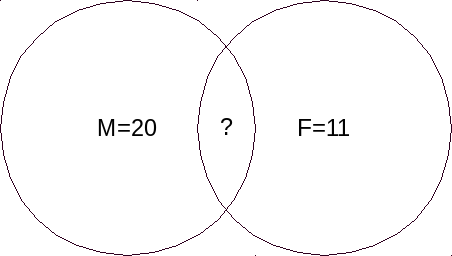
\includegraphics[width=.4\textwidth]{./pictures/1_14.png}
  \caption{Диаграмма Эйлера-Венна для задачи 1.14}
  \label{fig:114}
\end{figure}

Найдём, сколько учеников занимается хотя бы в одном кружке.
Это будет $35-10=25$ учеников.
Это есть количество элементов объединения двух множеств:
$$ |M \cup F| =
|M| + |F| - |M \cap F| =
25.$$
Отсюда можем найти, сколько учеников посещают и математический, и физический кружки:
$$ |M \cap F| =
|M| + |F| - |M \cup F| =
20 + 11 - 25 = 6.$$
Только математический кружок посещает $ |M| - |M \cap F| = 20 - 6 = 14$ учеников.

\addcontentsline{toc}{section}{Дополнительные задачи}
\section*{Дополнительные задачи}

\subsubsection*{1.15}

\textit{Задание.} Пусть множество X содержит n элементов, а множество Y --- m элементов.
Вычислить:

а) количество функций из X в Y;

б) количество инъекций из X в Y $\left(n\leq m\right)$;

в) количество биекций из X в Y $\left(n=m\right)$.

\textit{Решение.}

а) Можно считать, что $ X = \{1,  \dotsc , n \}, Y = \{1,  \dotsc , m \}$.
Каждую функцию можно отождествлять с последовательностью $ < f(1),  \dotsc , f(n) ) > = < y_1,  \dotsc , y_n > $.
Каждый член $y_i$ последовательности можно выбрать m способами, что даёт $m^n$ возможностей выбора $ < y_1,  \dotsc , y_n > $.

б) Будем определять число инъективных (то есть имеющих все различные члены) последовательностей $ < y_1,  \dotsc , y_n > $.
Элемент $y_1$ может быть выбран m способами, элемент $y_2$ можно выбрать $m-1$ способом из оставшихся элементов.
Если уже выбраны элементы $ y_1,  \dotsc , y_{i-1} $,
то в качестве $y_i$ может быть выбран любой из $m-i+1$ элементов множества
$Y\setminus\{y_1,  \dotsc , y_{i-1}\}$. Принимаем, что $ m \geq n $. если $ n > m $,
то искомое число функций равно 0.
Это даёт
$$m\left(m-1\right) \dotsc (m+n-1)
=\frac{m!}{\left(m-n\right)!}$$
возможность выбора инъективных последовательностей $<y_1,  \dotsc , y_n>$.

в) Если $n=m$, то любое инъективное отображение будет биективным.
Число всех биективных отражений X в Y равно $n!$ при $m = n$ и 0 при $m \neq n$.

\addcontentsline{toc}{section}{Домашнее задание}
\section*{Домашнее задание}

\subsubsection*{1.16}

\textit{Задание.} Подсчитать, сколько трёхзначных чисел можно записать с помощью:
а) цифр 0, 1, 2, 3, 4, 5;
б) цифр 0, 1, 2, 3, 4, 5, если каждую из цифр использовать не больше одного раза.

\textit{Решение.} Трёхзначное число можно рассматривать как трёхмерный вектор.
Первой компонентой этого вектора может быть любая цифра из множества
$$ A_1 = \{ 1, 2, 3, 4, 5 \} $$
(запись числа не может начинаться с 0).

а) На остальных позициях может стоять любая цифра, то есть
$$ A_i = \{ 0, 1, 2, 3, 4, 5 \}, i = 2, 3.$$
Отсюда имеем, что из указанных цифр можно составить $ 5 \cdot 6 \cdot 6 = 180$ трёхзначных чисел.

б) На остальных позициях могут стоять любые цифры (кроме тех, что стояли на предыдущих позициях).
Отсюда имеем, что из указанных цифр можно составить $ 5 \cdot 5 \cdot 4 = 100 $ трёхзначных чисел.

\subsubsection*{1.17}

\textit{Задание.} Подсчитать количество пятизначных чисел, которые делятся на 5.

\textit{Решение.} Пятизначное число можно рассматривать как пятимерный вектор.
Первой компонентой этого вектора может быть любая цифра из множества
$$ A_1 = \{ 1, 2, 3, 4, 5, 6, 7, 8, 9 \} $$
(запись числа не может начинаться с 0), а на остальных позициях (кроме последней) может стоять любая цифра, то есть
$$ A_i = \{ 0, 1, 2, 3, 4, 5, 6, 7, 8, 9 \}, i = 2, 3, 4.$$
На последней позиции может стоять цифра из множества $ A_5 = \{ 0, 5 \}$ (чтобы число делилось на 5, оно должно оканчиваться на 0 или 5).
Отсюда имеем, что можно составить $ 9 \cdot 10 \cdot 10 \cdot 10 \cdot 2 = 18000$ пятизначных чисел, которые делятся на 5.

\subsubsection*{1.18}

\textit{Задание.} Замок компьютерного центра состоит из пяти кнопок, пронумерованных от 1 до 5.
Чтобы открыть замок, необходимо первые две определённые кнопки нажать одновременно, а потом одну за другой нажать другие три кнопки в определённой последовательности. Подсчитать количество способов закодировать вход в компьютерный центр.

\textit{Решение.} Рассмотрим 3 случая: 

а) сначала необходимо нажать две разные кнопки, далее их отпускают, и все остальные кнопки могут быть любыми; 

б) первые две кнопки держатся нажатыми, следующие кнопки не могут быть такими, как первые две; 

в) нельзя нажать одну и ту же кнопку больше одного раза (кнопки остаются нажатыми).

Количество способов нажать первые две кнопки равна количеству двухэлементных подмножеств в множестве из пяти элементов, то есть
$$ C_5^2 = \frac{5!}{2! \left( 5 - 2 \right)!} = 10.$$

В случае а) количество способов закодировать вход в компьютерный центр равно
$$ C_5^2 \cdot 5^3 = 1250.$$
Общая формула: $ C_N^n \cdot N^m $, где N --- количество кнопок, n кнопок нажимаются вместе, а затем m кнопок --- по очереди.

В случае б) после нажатия двух кнопок, остаётся только 3 кнопки, которые необходимо нажать в правильном порядке,
поэтому количество способов по предыдущей формуле равно
$$ C_5^2 \cdot 3^3 = 270.$$

В случае в) все кнопки должны быть нажаты один раз, поэтому количество способов закодировать вход равно
$$ C_5^2 \cdot 3 \cdot 2 \cdot 1 = 60.$$

\subsubsection*{1.19}

\textit{Задание.} Колоду игральных карт (52 карты, 4 масти по 13 карт в каждой) тщательно перетасовали.
Подсчитать количество способов выбрать из неё 6 карт без возвращения так, чтобы среди них:
а) был пиковый король;
б) были представители всех мастей;
в) было ровно 5 карт одной масти.

\textit{Решение.}

а) Выбрать пикового короля есть только один способ.
Остальные 6 карт могут быть любыми из оставшихся 51 карты.
Выбрать эти 5 карт можно $ C_{51}^5 $ способами.
Отсюда имеем, что из колоды можно выбрать 6 карт, среди которых был бы пиковый король, $ 1 \cdot C_{51}^5 $ числом способов.

б) Сначала выберем по одной карте каждой масти.
Количество способов выбрать одну карту определённой масти равно $C_{13}^1$, так как имеется 13 карт каждой масти.
Так как всего есть 4 масти, то нужно выбрать 4 карты (по одной карте каждой масти).
Тогда количество способов выбрать 4 карты разных мастей равно
$$ C_{13}^1 \cdot C_{13}^1 \cdot C_{13}^1 \cdot C_{13}^1 =
\left( C_{13}^1 \right)^4.$$
Остаётся выбрать две произвольные карты из оставшихся.
После выбора четырёх карт разных мастей в колоде осталось $ 52 - 4 = 48 $ карт.
Число способов выбрать из них две карты равно $ C_{48}^2 $.
Отсюда имеем, что количество способов выбрать из данной колоды 6 карт без возвращения таким образом, чтобы среди них были представители всех мастей, равно
$$ \left( C_{13}^1 \right) \cdot C_{48}^2.$$

в) Сначала нужно выбрать 5 карт одной масти.
В одной масти 13 карт, следовательно число способов выбрать 5 карт одной масти равно $ C_{13}^5 $.
Так как всего мастей 4, и нам не важно, какой именно масти будут 5 вытянутых карт (главное, чтобы одной), то число способов будет равно
$$ 4 \cdot C_{13}^5.$$
Шестая карта должна быть любой, но отличатся с предыдущими пятью мастью, то есть её можно выбрать из $ 52 - 13 = 39 $ карт.
Число способов это сделать равно $ C_{39}^1 $.
Отсюда имеем, что число способов выбрать из колоды карт 6 карт так, чтобы среди них было ровно 5 карт одной масти, равно
$$ 4 \cdot C_{13}^5 \cdot C_{39}^1.$$

\subsubsection*{1.20}

\textit{Задание.} Сколькими способами можно разместить 10 одинаковых открыток в 4 почтовых ящиках так, чтобы:
а) не было пустых ящиков;
б) во втором ящике было 3 открытки.

\textit{Решение.}

а) Рассмотрим случай, когда в каждый ящик должна быть помещена хотя бы одна открытка.
Используем метод перегородок.
Выложим открытки в ряд.
Для определения расклада открыток по четырём почтовым ящикам разделим ряд тремя перегородками на 4 группы:
первая группа для первого ящика, вторая --- для второго и так далее.
Таким образом, число вариантов раскладки открыток по ящикам равно числу способов разложения трёх перегородок.
Перегородки могут стоять на любом из 9 мест (между 10 открытками --- 9 промежутков).
Поэтому число возможных расположений равно $ C_9^3 $.

б) Рассмотрим случай, когда во второй ящик должны быть помещены 3 открытки.
Поскольку открытки одинаковые, то во второй ящик можно сразу положить 3 открытки.
В этом случае нужно распределить $ 10 - 3 = 7$ одинаковых открыток между тремя почтовыми ящиками.

Используем метод перегородок.
Рассмотрим ряд из 9 предметов: 7 одинаковых открыток и 2 одинаковые перегородки, расположенных в произвольном порядке.
Каждый такой ряд однозначно соответствует некоторому способу раскладки открыток по ящикам:
в первый ящик попадают открытки, расположенные левее первой перегородки,
во второй --- расположенные между первой и второй перегородками и т.д. (между какими-то перегородками открыток может и не быть).
Поэтому число способов раскладки открыток по ящикам равно числу различных рядов из 7 открыток и 2 перегородок,
т.е равно $ C_9^2 $ (ряд определяется теми двумя местами из 9, на которых стоят перегородки).

\subsubsection*{1.21}

\textit{Задание.} Сколькими способами можно распределить 10 путёвок среди 10 студентов (по одной каждому), если: а) все путёвки разные; б) есть 4 путёвки одного типа и 6 --- другого?

\textit{Решение.}

а) Количество возможных перестановок 10 разных путёвок равно $10!$.

б) Если будем считать все 10 элементов перестановки с повторениями различными, то всего различных вариантов перестановок 10 путёвок ---
$$ ( 4 + 6 )! = 10!.$$
Однако среди этих перестановок не все различны.
Все путёвки одного типа можно переставлять местами друг с другом, и от этого перестановка не изменится.
Точно так же, можем переставлять путёвки другого типа.
Таким образом, перестановка может быть записана $4!6!$ способами.
Следовательно, число различных перестановок с повторениями равно
$$ \frac{ ( 4 + 6 )! }{ 4!6! } = \frac{10!}{4!6!}.$$

\subsubsection*{1.22}

\textit{Задание.} Доказать, что количество неубывающих путей на r-мерной целочисленной решётке
$$ \mathbb{Z}_+^r = \{ \left( i_1,  \dotsc , i_r \right) : i_1,  \dotsc , i_r = 0, 1, 2,  \dotsc \} ,$$
которые начинаются в точке $ \left( 0,  \dotsc , 0 \right) $ и приводят в точку $ \left( n_1,  \dotsc , n_r \right) $, равно
$$ C_N \left( n_1,  \dotsc , n_r \right) =
\frac{N!}{n_1! \dotsc n_r!},$$
где $ N = \sum \limits_{ i = 1 }^r n_i$.
(Путь считается неубывающим, если на каждом шаге изменяется только одна координата, увеличиваясь на единицу.)

\textit{Решение.} Имеем пути, состоящие из $ n_1 + \dotsc + n_r$ ходов,
среди которых ровно $n_1$ ходов в направлении $ r_1$,  $\dotsc$ , и $n_r$ ходов в направлении $r_n$.
Если выберем, на каких шагах увеличиваем первую координату, будем знать, где увеличиваем остальные координаты.
Далее выберем, на каких шагах увеличиваем вторую координату.
И так необходимо определить, где увеличиваем $ n_1+ \dotsc n_{r-1}$ координат.
Тогда будем однозначно знать, где увеличиваем последнюю координату.
Это будет
$$ \frac{ \left( n_1 + \dotsc + n_r \right) }{ n_1! \dotsc n_r! }.$$

\subsubsection*{1.23}

\textit{Задание.} Из 100 студентов английский язык знают 28,
немецкий --- 30, французский --- 42, английский и немецкий --- 8, английский и французский --- 10, немецкий и французский --- 5, а все три языка знают 3 студента.
Сколько студентов не знают ни одного языка?

\textit{Решение.} Условие задачи представлено на рисунке \ref{fig:123} в виде диаграммы Эйлера-Венна. 

\begin{figure}[h!]
  \centering
  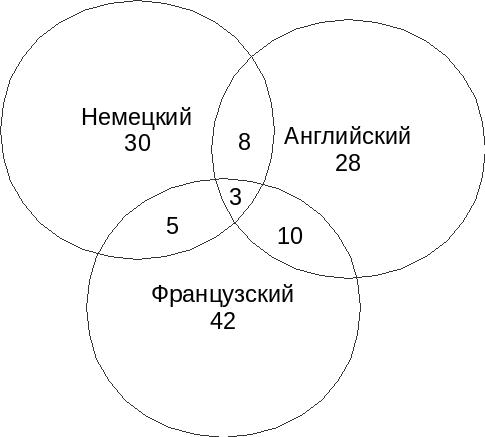
\includegraphics[width=.4\textwidth]{./pictures/1_23.png}
  \caption{Диаграмма Эйлера-Венна для задачи 1.23}
  \label{fig:123}
\end{figure}

Сначала найдём, сколько студентов знает хотя бы один язык.
Это есть мощность (количество элементов) объединения трёх множеств: Английский, Немецкий и Французский, которые обозначим первыми буквами.
Мощность объединения трёх множеств можно найти как сумму мощностей этих множеств, но, так как они пересекаются,
необходимо отнять мощности их пересечений и добавить пересечение всех трёх множеств, потому что его отняли дважды.
Имеем
\begin{equation*}
\begin{split}
|H \cup A \cup F| =
|H| + |A| + |F| - |H \cap A| - |A \cap F| - |H \cap F| + |H \cap A \cap F| = \\
= 30 + 42 + 28 - 5 - 8 - 10 + 3 = 80.
\end{split}
\end{equation*}

Все остальные студенты из ста не знают ни одного языка.
Их 
$$ 100 - 80 = 20.$$

\addcontentsline{toc}{chapter}{Занятие 2. События и операции над ними. Пространство элементарных событий}
\chapter*{Занятие 2. События и операции над ними. Пространство элементарных событий}

\addcontentsline{toc}{section}{Контрольные вопросы и задания}
\section*{Контрольные вопросы и задания}

\subsubsection*{Приведите определение вероятностного эксперимента, вероятностного пространства, случайного события.}

Вероятностным экспериментом называется явление, исход которого для нас не определён, и которое можно повторить любое число раз независимым образом.

Вероятностное пространство --- совокупность всех исходов вероятностного эксперимента, $ \Omega $.

Случайное событие --- подмножество всех исходов вероятностного эксперимента, $ A \subset \Omega $.

\subsubsection*{Запишите основные операции над случайными событиями и дайте их теоретико-множественную интерпретацию.}

Операции будем иллюстрировать на диаграммах Эйлера-Венна.
На рис.\ref{fig:2} заштрихованы области, которые соответствуют событиям, являющимся результатами таких операций.

Пересечением (произведением) двух событий А и В называют событие С, происходящее тогда и только тогда,
когда одновременно происходят оба события А и В, т.е событие,
состоящее из тех и только тех элементарных исходов, которые принадлежат и события А, и событию В (рис.\ref{fig:2}, а).

Пересечение событий А и В записывают следующим образом: $ C = A \cap B $, или $ C = AB $.

События А и В называют несовместимыми, или непересекающимися, если их пересечение является невозможным событием, т.е если $ A \cap B = \varnothing$ (рис.\ref{fig:2}, б).

В противном случае события называют совместимыми, или пересекающимися.

\begin{figure}[h!]
  \centering
  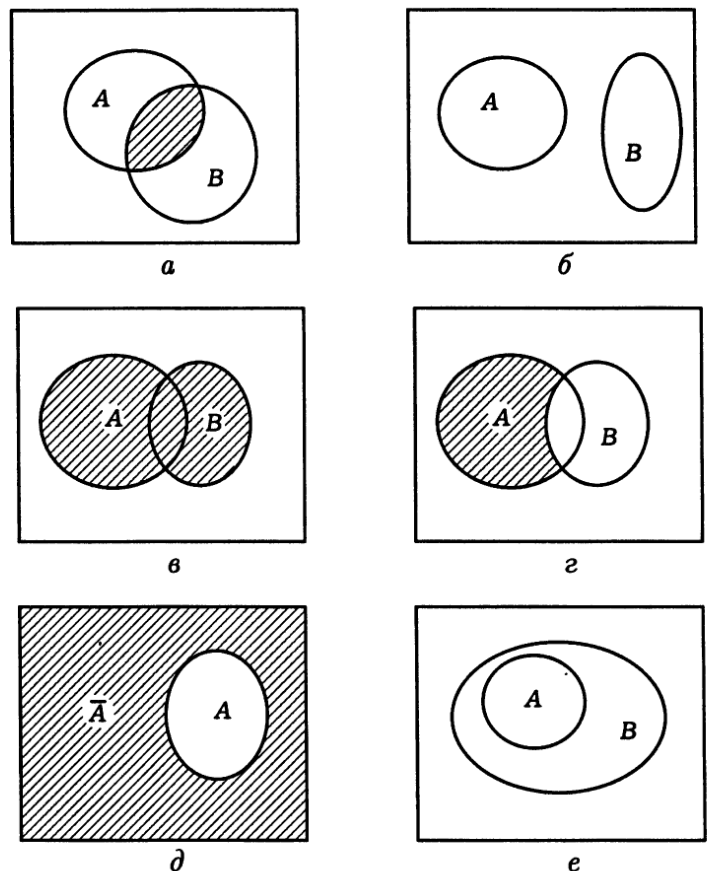
\includegraphics[width=.7\textwidth]{./pictures/2.png}
  \caption{Диаграммы Эйлера-Венна для операций над событиями}
  \label{fig:2}
\end{figure}

Объединением (суммой) двух событий А и В называют событие С,
происходящее тогда и только тогда,
когда происходит хотя бы одно из событий А или В, т.е.
событие С, состоящее из тех элементарных исходов, которые принадлежат хотя бы одному из подмножеств А или В (рис.\ref{fig:2}, в).

Объединение событий А и В записывают в виде $ C = A \cup B $.

Разностью двух событий А и В называют событие С,
происходящее тогда и только тогда,
когда происходит событие А,
но не происходит событие В, т.е. событие С, состоящее из тех элементарных исходов, которые принадлежат А, но не принадлежат В (рис.\ref{fig:2}, г).

Разность событий А и В записывают в виде: $ C = A \setminus B $.

Дополнением события А (обычно обозначают $ \overline{A} $) называют событие, происходящее тогда и только тогда, когда не происходит событие А (рис.\ref{fig:2}, д).
Другими словами, $ \overline{A} = \Omega \setminus A $.

Событие А включено в событие В,
что записывается $ A \subset B $,
если появление события А обязательно влечёт за собой наступление события В (рис.\ref{fig:2}, е),
или каждый элементарный исход $ \omega $, принадлежащий А, обязательно принадлежит и событию В.

Верхний предел последовательности $ \{ A_n : n \geq 1 \} $ --- это случайное событие,
состоящее в том, что произошло бесконечно много событий из исходной последовательности:
$$ \varlimsup \limits_{ n \to \infty } A_n =
\bigcap \limits_{n \geq 1} \bigcup \limits_{ m \geq n } A_m.$$

$ \forall n \exists m \geq n : A_m $ произошло.

Нижний предел последовательности:
$ \{ A_n : n \geq 1 \} $ --- это случайное событие, состоящее в том, что произошли все события, начиная с некоторого из исходной последовательности:
$$ \varliminf \limits_{ n \to \infty } A_n =
\bigcup \limits_{ n = 1 }^\infty \bigcap \limits_{ m = n }^\infty A_m.$$

$ \exists n \forall m \geq n $ происходит событие $A_m$.

\subsubsection*{Сформулируйте законы де Моргана.}

Первый закон де Моргана гласит: <<Если неверно, что есть и первое, и второе, то неверно либо одно из, либо оба>>, что выражается следующей формулой:
$ \overline{ AB } = \overline{ A } \cup \overline{ B }$.

Второй закон де Моргана гласит: <<Если неверно, что есть первое, или неверно, что есть второе, то неверно, что есть первое и второе>>, что выражается следующей формулой:
$ \overline{ A \cup B} = \overline{ A }$ $ \overline{ B }$.

Законы де Моргана верны для любого конечного числа событий:
\begin{equation*}
\begin{split}
\overline{ A_1 \cup A_2 \cup \dotsc \cup A_n } =
\overline{ A_1 } \, \overline{ A_2 } \, \dotsc \overline{ A_n }, \\
\overline{ A_1 A_2 \dotsc A_n } =
\overline{ A_1 } \cup \overline{ A_2 } \cup \dotsc \cup \overline{ A_n }.
\end{split}
\end{equation*}

\addcontentsline{toc}{section}{Аудиторные задачи}
\section*{Аудиторные задачи}

\subsubsection*{2.3}

\textit{Задание.} Рассмотрим эксперимент, который состоит в подбрасывании трёх монет.
Постройте множество $ \Omega $ элементарных событий этого эксперимента.
Опишите событие A, которое состоит в том, что выпало не меньше двух гербов.
Вычислите вероятность события A.

\textit{Решение.} Пусть эксперимент состоит в подбрасывании одной монеты.
При математическом описании этого опыта естественно отвлечься от несущественных возможностей
(например, монета встанет на ребро) и ограничиться только двумя элементарными исходами:
выпадение <<герба>> (обозначим этот исход $ \omega_1 $) и выпадением <<цифры>> (обозначим этот исход $\omega_2$).
Таким образом, $ \Omega_1 = \{ \omega_1, \omega_2 \} $.

При подбрасывании двух монет пространство элементарных исходов будет содержать три элемента,
т.е. $ \Omega_2 = \{ \omega_{11}, \omega_{12}, \omega_{22} \} $, где, например, $\omega_{11}$ --- появление <<герба>> и на первой, и на второй монете.

При подбрасывании трёх монет пространство элементарных исходов будет содержать элементов, т.е.
$ \Omega_3 = \Omega = \{ \omega_{111}, \omega_{112}, \omega_{122}, \omega_{222} \} $, где, например,
$ \omega_{111} $ --- появление <<герба>> и на первой, и на второй, и на третьей монете.

Событие A состоит в том, что выпало не меньше двух гербов, т.е. два или три герба.
Выберем из $ \Omega $ такие исходы: $ A = \{ \omega_{122}, \omega_{222} \} $.

Поскольку $ |A| = 2, | \Omega | = 4$, то
$$ P(A) = \frac{ |A| }{| \Omega |} =
\frac{2}{4} =
\frac{1}{2}.$$

\subsubsection*{2.4}

\textit{Задание.} Пусть A, B, C --- произвольные события.
Найдите выражения для событий, который состоят в том, что из событий A, B и C:

а) произошло только  A;

б) произошли A и B, но не произошло C;

в) произошли все три события;

г) произошло хотя бы одно из этих событий;

д) произошло хотя бы два события;

е) произошло одно и только одно событие;

ё) произошло два и только два события;

ж) ни одно из событий не произошло;

з) произошло не больше двух событий.

\textit{Решение.}

а) $ A \cap \overline{ B } \, \overline{ C } $;

б) $ A \cap B \cap \overline{ C } $;

в) $ A \cap B \cap C $;

г) $ A \cup B \cup C $;

д) $ \left( A \cap B \right) \cup \left( A \cap C \right) \cup \left( B \cap C \right) $;

е) $ \left( A \cap \overline{ B } \cap \overline{ C } \right) \cup \left( B \cap \overline{ A } \cap \overline{ C } \right)
\cup \left( C \cap \overline{ A } \cap \overline{ B } \right) $;

ё) $ \left( A \cap B \cap \overline{ C } \right) \cup \left( A \cap C \cap \overline{ B } \right) \cup \left( B \cap C \cap \overline{ A } \right) $;

ж) $ \overline{ A } \cap \overline{ B } \cap \overline{ C } $;

з) $ \left( \overline{ A } \cap \overline{ B } \cap \overline{ C } \right) \cup
\left( A \cap \overline{ B } \cap \overline{ C } \right) \cup
\left( B \cap \overline{ A } \cap \overline{ C } \right) \cup
\left( C \cap \overline{ A } \cap \overline{ B } \right) \cup
\left( A \cap B \cap \overline{ C } \right) \cup \\
\cup \left( A \cap C \cap \overline{ B } \right) \cup
\left( B \cap C \cap \overline{ A } \right)$.

\subsubsection*{2.5}

\textit{Задание.} Пусть A и B --- некоторые события.
Упростите выражение
$$ C = \overline{ \overline{ A \cap \overline{ B } } \cup \overline{ A \cup B } \cup \left( B \cap A \right) }.$$

\textit{Решение.}
$ C =
\overline{ \overline{ A \cap \overline{ B }}} \cup \overline{ \overline{ A \cup B }} \cup \overline{ B \cap A } =
\left( A \cap \overline{ B } \right) \cup A \cup B \cup \overline{ B } \cup \overline{ A } = \\
= \left( A \cap \overline{ B } \right) \cup A \cup \overline{ A } \cup B \cup \overline{ B } =
\left( A \cap \overline{ B } \right) \cup \Omega \cup \Omega =
\left( A \cap \overline{ B } \right) \cup \Omega =
\Omega $.

\subsubsection*{2.6}

\textit{Задание.} Пусть $ \{ A_n, n \in \mathbb{N} \}, \{ B_n, n \in \mathbb{N} \} $ --- некоторые последовательности событий.
Объясните, что значат события $ \varlimsup \limits_{n \to \infty } A_n, \varliminf \limits_{n \to \infty } A_n$.
Докажите, что:

а) $ \overline{ \varlimsup \limits_{ n \to \infty } A_n } =
\varliminf \limits_{ n \to \infty } \overline{ A_n }$;

б) $ \varlimsup \limits_{ n \to \infty } \left( A_n \cup B_n \right) =
\varlimsup \limits_{ n \to \infty } A_n \cup \varlimsup \limits_{ n \to \infty } B_n $.

\textit{Решение.} Верхний предел последовательности $ \{ A_n : n \geq 1 \} $ ---
это случайное событие, состоящее в том, что произошло бесконечно много событий из исходной последовательности:
$$ \varlimsup \limits_{ n \to \infty } A_n =
\bigcap \limits_{ n \geq 1 } \bigcup \limits_{ m \geq n} A_m.$$

$ \forall n \exists m \geq n : A_m $ произошло.

Нижний предел последовательности:
$ \{ A_n : n \geq 1 \}$ --- это случайное событие, состоящее в том, что произошли все события, начиная с некоторого из исходной последовательности:
$$ \varliminf \limits_{ n \to \infty } A_n =
\bigcup \limits_{ n = 1 }^\infty \bigcap \limits_{ m = n }^\infty A_m.$$

$ \exists n \forall m \geq n $ происходит событие $A_m$.

а) $\overline{ \varlimsup \limits_{ n \to \infty } A_n } =
\overline{ \bigcap \limits_{ n \geq 1} \bigcup \limits_{ m \geq n} A_m } =
\bigcup \limits_{ n \geq 1} \overline{ \bigcup \limits_{ m \geq n} A_m } =
\bigcup \limits_{ n \geq 1} \bigcap \limits_{ m \geq n} \overline{ A_m } =
\varliminf \limits_{ n \to \infty} \overline{ A_n }$;

б) $\varlimsup \limits_{ n \to \infty } \left( A_n \cup B_n \right) =
\bigcap \limits_{ n \geq 1} \bigcup \limits_{ m \geq n} \left( A_m \cup B_m \right) =
\prod \limits_{ n = 1 }^\infty \sum \limits_{ m = n }^\infty \left( A_m + B_m \right) = \\
= \prod \limits_{ n = 1 }^\infty \sum \limits_{ m = n }^\infty A_m + \prod \limits_{ n = 1 }^\infty \sum \limits_{ m = n }^\infty B_m =
\varlimsup \limits_{ n \to \infty } A_n \cup \varlimsup \limits_{ n \to \infty } B_n $.

\subsubsection*{2.7}

\textit{Задание.} Пусть $ \{ A_n, n \in \mathbb{N} \} $ --- некоторая последовательность событий, $ \mathbbm{1} ( A ) $ --- индикатор события A.
Докажите, что $ \mathbbm{ 1 } \left( \varlimsup \limits_{ n \to \infty } A_n \right) =
\varlimsup \limits_{ n \to \infty } \mathbbm{ 1 } \left( A_n \right) $.

\textit{Решение.} Рассмотрим 4 случая: 

\begin{enumerate}
\item $ \mathbbm{ 1 } \left( \varlimsup \limits_{ n \to \infty } A_n \right) = 0,
\varlimsup \limits_{ n \to \infty } \mathbbm{ 1 } \left( A_n \right) = 0 $;
\item $ \mathbbm{ 1 } \left( \varlimsup \limits_{ n \to \infty } A_n \right) = 0,
\varlimsup \limits_{ n \to \infty } \mathbbm{ 1 } \left( A_n \right) = 1 $;
\item $ \mathbbm{ 1 } \left( \varlimsup \limits_{ n \to \infty } A_n \right) = 1,
\varlimsup \limits_{ n \to \infty } \mathbbm{ 1 } \left( A_n \right) = 0 $;
\item $ \mathbbm{ 1 } \left( \varlimsup \limits_{ n \to \infty } A_n \right) = 1,
\varlimsup \limits_{ n \to \infty } \mathbbm{ 1 } \left( A_n \right) = 1 $.
\end{enumerate}

Нужно доказать, что возможны только первый и последний случаи.

Верхний предел последовательности
$ \{ A_n : n \geq 1 \} $ --- это случайное событие, состоящее в том, что произошло бесконечно много событий из исходной последовательности:
$$ \varlimsup \limits_{ n \to \infty } A_n =
\bigcap \limits_{ n \geq 1} \bigcup \limits_{ m \geq n} A_m.$$

Индикатор --- функция двух переменных:
$ \mathbbm{1} \left( \omega, A \right) $,
где $\omega$ --- элементарный исход (то, что произошло), A --- случайное событие (то, что рассматриваем).
Если $\omega \in A$, то индикатор равен 1, иначе --- 0.

Индикатор верхнего предела равен нулю
$ \left( \mathbbm{ 1 } \left( \varlimsup \limits_{ n \to \infty } A_n \right) = 0 \right)$ --- значит, произошло конечное множество событий из $A_n$.
Значит, с какого-то момента события перестали происходить, и предел индикаторов равен нулю: $ \varlimsup \limits_{ n \to \infty } \mathbbm{ 1 } \left( A_n \right) = 0$.

Если индикатор от верхнего предела равен единице
$$ \left( \mathbbm{ 1 } \left( \varlimsup \limits_{ n \to \infty } A_n \right) =
\mathbbm{ 1 } \left( \bigcap \limits_{ n \geq 1} \bigcup \limits_{ m \geq n } A_m \right) =
1 \right) ,$$
то произошло бесконечное множество событий из $A_n$.
Это значит, во-первых, что пересечение не пустое, а во-вторых, что элементарный исход принадлежит этому пересечению.
Верхний предел последовательности событий --- это такое случайное событие,
что каждый случайный исход из него принадлежит бесконечному количеству событий из последовательности.
Поэтому
$ \varlimsup \limits_{ n \to \infty } \mathbbm{ 1 } \left( A_n \right) = 1 $.

\subsubsection*{2.8}

\textit{Задание.} Пусть B и C --- два события.
Положим $ A_n = B $, если n чётное и $ A_n = C $, если n нечётное.
Найдите событие, которое состоит в том, что:

а) произошло бесконечно много событий из последовательности $ \{ A_n \}_{ n = 1 }^\infty $;

б) произошло только конечное количество событий из последовательности $ \{ A_n \}_{ n = 1 }^\infty $.

\textit{Решение.}

а) По определению $ \varlimsup \limits_{ n \to \infty } A_n = \bigcap \limits_{ n \geq 1} \bigcup \limits_{ m \geq n} A_m $.

При $ n = 1: \bigcup \limits_{ m \geq 1} A_m = A_1 \cup A_2 \cup A_3 \cup \dotsc = B \cup C $.
Пересечение бесконечного количества одинаковых множеств даёт $ \varlimsup \limits_{ n \to \infty } A_n = B \cup C $;

б) по определению $ \varliminf \limits_{ n \to \infty } A_n = \bigcup \limits_{ n = 1 }^\infty \bigcap \limits_{ m = n }^\infty A_m = B \cap C $.

При $ n = 1 : \bigcap \limits_{ m \geq 1 } A_m = A_1 \cap A_2 \cap A_3 \cap \dotsc = B \cap C $, поэтому $ \varliminf \limits_{ n \to \infty } A_n = B \cap C $.

\subsubsection*{2.9}

\textit{Задание.} Рассмотрим эксперимент, который состоит в выборе наугад точки в квадрате с вершинами в точках $ A(0, 0), B(0, 1), C(1, 1) $ и $ D(1, 0) $.
Опишите и изобразите вероятностное пространство этого эксперимента и следующие события:

а) A = {данная точка оказалась на расстоянии не меньшем чем 1/4 от сторон квадрата};

б) B = {данная точка оказалась внутри круга с центром в начале координат и радиусом 1/2};

в) $ \overline{ A }, \overline{ B }, A \cap B $.

\textit{Решение.} Пространство элементарных событий ( \ref{fig:29}, а)) опишем как множество упорядоченных пар
$ \Omega = \{ (x, y), 0 \leq x \geq 1, 0 \leq y \geq 1 \} $, где x --- первая координата точки, y --- вторая координата точки.

\begin{figure}[h!]
  \centering
  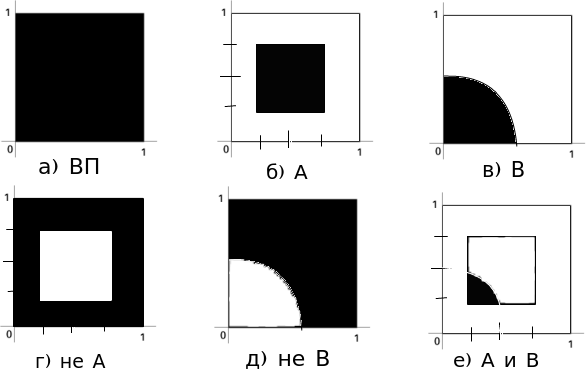
\includegraphics[width=.7\textwidth]{./pictures/2_9.png}
  \caption{Вероятностное пространство и события из задачи 2.9}
  \label{fig:29}
\end{figure}

а) $ A = \{ (x, y), \frac{3}{4} \leq x \geq \frac{1}{4}, \frac{3}{4} \leq y \geq \frac{1}{4}, \} $ ( \ref{fig:29}, б));

б) $ B = \{ (x, y), x \geq 0, y \geq 0, x^2 + y^2 \leq \frac{1}{2} \} $ ( \ref{fig:29}, в));

в) событие $ \overline{ A } $ означает, что событие A не произошло, то есть расстояние от точки до сторон квадрата оказалось больше 1/4 ( \ref{fig:29}, г)):
$$ \overline{ A } =
\{ (x, y), \frac{3}{4} > x > \frac{1}{4},
\frac{3}{4} > y > \frac{1}{4} \}.$$

Событие $ \overline{ B } $ означает, что данная точка не оказалась внутри круга с центром в начале координат и радиусом 1/2 ( \ref{fig:29}, д)):
$$ \overline{ B } =
\{ (x, y),
\frac{1}{2} > x^2 + y^2 \leq 1,
x \leq 1,
y \leq 1. \} $$

Событие $ A \cap B $ означает, что произошло и событие A, и событие B ( \ref{fig:29}, е)).
Отсюда имеем, что данная точка оказалась на расстоянии не меньшем чем 1/4 от сторон квадрата, а так же внутри круга с центром в начале координат и радиусом 1/2, т.е.
$$ A \cap B =
\{ (x, y),
x \geq \frac{1}{4},
y \geq \frac{1}{4},
x^2 + y^2 \leq \frac{1}{2} \}.$$

\addcontentsline{toc}{section}{Дополнительные задачи}
\section*{Дополнительные задачи}

\subsubsection*{2.10}

\textit{Задание.} Пусть A --- множество из n элементов,
$ A_1,  \dotsc , A_k $ --- подмножества A такие, что ни одно из подмножеств не является частью другого,
а $ i_1,  \dotsc , i_k $ --- количество элементов подмножеств $ A_1,  \dotsc , A_k $ соответственно.
Докажите, что
$$ \sum \limits_{ r = 1 }^k \frac{ 1 }{ C_n^{ i_r } } \leq 1.$$

\textit{Решение.} Умножим слева и справа на произведение знаменателей:
$$ \prod \limits_{r=1}^k C_n^{i_r} \sum \limits_{r=1}^k \frac{1}{C_n^{i_r}} \leq
\prod \limits_{r=1}^k C_n^{i_r}. $$

Внесём произведение под знак суммы:
$$ \sum \limits_{r=1}^k \frac{ \prod \limits_{r'=1}^k C_n^{i_{r'}}}{C_n^{i_r}} \leq
\prod \limits_{r=1}^k C_n^{i_r}. $$

Упростим:
$$ \sum \limits_{r=1}^k \prod \limits_{1 \leq r' \leq k}^{r' \neq r} C_n^{i_{r'}} \leq
\prod \limits_{r=1}^k C_n^{i_r}. $$

Обозначим номер наибольшего слагаемого как r:
$$ m = arg \max \limits_{1 \leq r \leq k} \prod \limits_{1 \leq r' \leq k}^{r' \neq r} C_n^{i_{r'}}. $$

Сумма слагаемых не больше чем наибольшее из них взятое k раз, т.е.
$$ \sum \limits_{r=1}^k \prod \limits_{1 \leq r' \leq k}^{r' \neq r} C_n^{i_{r'}} \leq
k \cdot \prod \limits_{1 \leq r' \leq k}^{r' \neq m} C_n^{i_{r'}} \leq
\prod \limits_{r=1}^k C_n^{i_r}. $$

Поделим правую и левую часть полученного неравенства на произведение, стоящее в левой части:
$$ k \leq
\frac{ \prod \limits_{r=1}^k C_n^{i_r}}{ \prod \limits_{1 \leq r' \leq k}^{r' \neq m} C_n^{i_{r'}}} =
C_n^m. $$

Если $ k \leq n $, то неравенство выполняется для любого возможного m кроме $ m = 0 $ и $ m = n $.

$ m = 0 $ возможно только если $A_1$ --- пустое множество и $k = 1$,
потому что если бы там были другие множества, пустое было бы их подмножеством, что противоречит условию задачи.
Тогда $ C_0^0 = 1 \leq 1$.

$ m = n $, то $ A_1 = A, k = 1 $, значит $C_n^n = 1$.
Если будут другие подмножества кроме $A_1$, то они будут подмножествами $A_1$, что противоречит условию.

\paragraph*{Формулы Стирлинга.}

Распишем левую часть неравенства:
$$ \sum \limits_{r=1}^k \frac{1}{C_n^{i_r}} =
\sum \limits_{r=1}^k \frac{1}{ \frac{n!}{i_{r}! \left(n-i_r\right)!} } =
\sum \limits_{r=1}^k \frac{i_{r}! \left(n-i_r\right)!}{n!}.$$

Получили неравенство:
$$\sum \limits_{r=1}^k \frac{i_{r}! \left(n-i_r\right)!}{n!} \leq 1.$$

Умножим левую и правую части неравенства на $n!$.
Левая часть:
$$ n! \cdot \sum \limits_{r=1}^k \frac{i_{r}! \left(n-i_r\right)!}{n!} =
\sum \limits_{r=1}^k i_{r}! \left(n-i_r\right)!.$$

Получили неравенство:
$$\sum \limits_{r=1}^k i_{r}! \left(n-i_r\right)! \leq n!. $$
Нижний и верхний пределы для факториала:
$$ \sqrt{2 \pi n} \left( \frac{n}{e} \right)^n \exp \left( \frac{1}{12 n+1} \right) <
n! <
\sqrt{2 \pi n} \left( \frac{n}{e} \right)^n \exp \left( \frac{1}{12 n} \right). $$

Возьмём для левой части неравенства верхний предел, а для правой --- нижний:
\begin{equation*}
\begin{split}
\sum \limits_{r=1}^k \sqrt{2 \pi i_r} \left( \frac{i_r}{e} \right)^{i_r} \exp \left( \frac{1}{12 i_r} \right)
\left( \frac{i_r}{e} \right)^{i_r} \sqrt{2 \pi  \left( n-i_r\right) }
\left( \frac{n-i_r}{e} \right)^{n-i_r} \times \\
\times \exp \left( \frac{1}{12 \left( n-i_r\right) } \right) \leq 
\sqrt{2 \pi n} \left( \frac{n}{e} \right)^n \exp \left( \frac{1}{12 n+1} \right).
\end{split}
\end{equation*}

Сократим на $ \sqrt{2 \pi } $ и упростим:
\begin{equation*}
\begin{split}
\sum \limits_{r=1}^k \sqrt{i_r \left( n-i_r \right) }
\exp \left( \frac{1}{12 i_r} + \frac{1}{12 \left( n-i_r \right) } \right) \left( \frac{i_r}{e} \right)^{i_r}
\left( \frac{n-i_r}{e} \right)^{n-i_r} \leq \\
\leq \sqrt{n} \left( \frac{n}{e} \right)^n \exp \left( \frac{1}{12 n+1} \right).
\end{split}
\end{equation*}

Упростим экспоненты в знаменателях левой части:
$$ \exp \left( - i_r \right) \exp \left( i_r - n \right) =
\exp \left( - i_r + i_r - n \right) =
\exp \left( -n \right).$$

В правой части имеем такую же степень экспоненты, поэтому сократим:
\begin{equation*}
\begin{split}
\sum \limits_{r=1}^k \sqrt{i_r \left( n-i_r \right) }
\exp \left( \frac{1}{12 i_r} + \frac{1}{12 \left( n-i_r \right) } \right) i_r^{i_r} \left( n-i_r \right)^{n-i_r} \leq \\
\leq \sqrt{n} n^n \exp \left( \frac{1}{12 n+1} \right).
\end{split}
\end{equation*}

Приведём подобные:
$$ \sum \limits_{r=1}^k i_r^{i_r + \frac{1}{2} } \left( n-i_r \right)^{n - i_r + \frac{1}{2} }
\exp \left( \frac{1}{12 i_r} + \frac{1}{12 \left( n-i_r \right) } \right) \leq
n^{n + \frac{1}{2} } \exp \left( \frac{1}{12 n+1} \right). $$

Приведём к общему знаменателю дроби в степени экспоненты в левой части:
$$ \frac{1}{12 i_r} + \frac{1}{12 \left( n-i_r \right) } =
\frac{n - i_r + i_r}{12 i_r \left( n-i_r \right) } =
\frac{n}{12 i_r \left( n-i_r \right) }. $$

Подставим в неравенство:
$$ \sum \limits_{r=1}^k i_r^{i_r + \frac{1}{2} } \left( n-i_r \right)^{n - i_r + \frac{1}{2} }
\exp \left( \frac{n}{12 i_r \left( n-i_r \right) } \right) \leq 
n^{n + \frac{1}{2} } \exp \left( \frac{1}{12 n+1} \right). $$

Упростим выражение в левой части так, что оно станет больше:
\begin{equation*}
\begin{split}
\sum \limits_{r=1}^k i_r^{i_r + \frac{1}{2} } n^{n - i_r + \frac{1}{2} }
\exp \left( \frac{n}{12 i_r \left( n-i_r \right) } \right) \leq \\
\leq n^{n + \frac{1}{2} } \exp \left( \frac{1}{12 n+1} \right).
\end{split}
\end{equation*}

Сократим на $ n^{n + \frac{1}{2} } $.
Получим:
$$ \sum \limits_{r=1}^k i_r^{i_r + \frac{1}{2} } \left( \frac{1}{n} \right)^{i_r}
\exp \left( \frac{n}{12 i_r \left( n-i_r \right) } \right) \leq
\exp \left( \frac{1}{12 n+1} \right). $$

Внесём $ i_r^{i_r} $ в числитель дроби и поделим на экспоненту из правой части:
$$ \sum \limits_{r=1}^k \sqrt{i_r} \left( \frac{i_r}{n} \right)^{i_r}
\exp \left( \frac{n}{12 i_r \left( n-i_r\right) } - \frac{1}{12 n + 1} \right) \leq 1. $$

Сведём дроби в степени экспоненты к общему знаменателю:
\begin{equation*}
\begin{split}
\frac{n}{12 i_r \left( n-i_r \right) } - \frac{1}{12 n + 1} =
\frac{n \left( 12 n + 1 \right) - 12 i_r \left( n-i_r \right) }{12 i_r \left( n-i_r \right) \left( 12 n + 1\right) } = \\
= \frac{12 n^2 + n - 12 i_r n + 12 i_r^2}{12 i_r \left( n-i_r \right) \left( 12 n + 1\right) } =
\frac{12 n^2 + n - 12 i_r n + 12 i_r^2}{ \left( 12 i_r n - 12 i_r^2 \right) \left( 12 n + 1 \right) } = \\
= \frac{12 n^2 + n - 12 i_r n + 12 i_r^2}{144 n^2 i_r + 12 i_r n - 144 i_r^2 n - 12 i_r^2} =
\frac{12 \left( n^2 -2 i_r n + i_r^2 \right) + n + 12 i_r n}{144 n^2 i_r + 12 i_r n - 144 i_r^2 n - 12 i_r^2} = \\
= \frac{12 \left( n-i_r\right)^2 + n + 12 i_r n }{144 n^2 i_r + 12 i_r n - 144 i_r^2 n - 12 i_r^2}.
\end{split}
\end{equation*}

Упростим выражение, используя нижний предел для количества сочетаний:
$$ \left( \frac{n}{k} \right)^k \leq C_n^k. $$

Получим:
$$\sum \limits_{r=1}^k \frac{1}{C_n^{i_r}} \leq
\sum \limits_{r=1}^k \frac{1}{\left( \frac{n}{i_r} \right)^{i_r}} =
\sum \limits_{r=1}^k \left( \frac{i_r}{n} \right)^{i_r}. $$

\addcontentsline{toc}{section}{Домашнее задание}
\section*{Домашнее задание}

\subsubsection*{2.11}

\textit{Задание.} Рассмотрим эксперимент, который состоит в подбрасывании трёх игральных кубиков.
Опишите множество $ \Omega $ элементарных событий этого эксперимента; из скольки элементарных событий оно состоит?
Опишите событие С, которое состоит в том, что на всех кубиках выпало одинаковое количество очков.
Вычислите вероятность события С.

\textit{Решение.} Пространство элементарных событий опишем как множество упорядоченных троек
$ \Omega = \{ \left( i, j, k \right),
i = \overline{ 1, 6 },
j = \overline{ 1, 6 },
k = \overline{ 1, 6 } \} $,
где i --- количество очков, которые выпали на первом кубике,
j --- количество очков, которые выпали на втором кубике,
k --- количество очков, которые выпали на третьем кубике.

Можем рассматривать тройку чисел как вектор длины 3.
Первой компонентой вектора может быть любое значение из $ \{ 1, 2, 3, 4, 5, 6 \} $.
Его можно выбрать $ C_6^1 = 6 $ способами.
Таким же образом находим, что есть 6 способов выбрать вторую компоненту вектора и 6 --- третью.
По правилу умножения имеем $ 6 \cdot 6 \cdot 6 = 6^3 = 108 $ разных векторов указанного вида, или элементарных событий.

$ C = \{ (1, 1, 1), (2, 2, 2), (3, 3, 3), (4, 4, 4), (5, 5, 5), (6, 6, 6) \} $.
Поскольку
$$ |C| = 6,
|\Omega| = 108, $$
то
$$ P(C) =
\frac{ |C| }{ |\Omega| } =
\frac{ 6 }{ 108 } =
\frac{ 1 }{ 36 }.$$

\subsubsection*{2.12}

\textit{Задание.} Монету подбрасывают до тех пор, пока она не выпадет 2 раза подряд одной и той же стороной, но не больше четырёх раз.
Опишите множество $ \Omega $ элементарных событий.
Опишите следующие события и вычислите их вероятности:

а) А = { эксперимент закончился на втором подбрасывании};

б) В = { эксперимент закончился на третьем подбрасывании};

в) C = { эксперимент закончился на четвёртом подбрасывании}.

\textit{Решение.}  Пусть опыт состоит в однократном подбрасывании монеты.
При математическом описании этого опыта естественно отвлечься от несущественных возможностей
(например, монета встанет на ребро) и ограничиться только двумя элементарными исходами:
выпадение <<герба>> (обозначим этот исход $ \omega_1 $) и выпадением <<цифры>> (обозначим этот исход $ \omega_2 $).
Таким образом, $ \Omega_1 = \{ \omega_1, \omega_2 \} $.

При двукратном подбрасывании монеты пространство элементарных исходов будет содержать четыре элемента, т.е.
$$ \Omega_2 = \{ \omega_{11}, \omega_{12}, \omega_{21}, \omega_{22} \},$$
где, например, $ \omega_{11} $ --- появление <<герба>> и при первом, и при втором подбрасываниях.
В данном случае эксперимент может завершиться, если при двукратном подбрасывании монеты она выпала два раза одной и той же стороной.
Поэтому $ A = \{ \omega_{11}, \omega_{22} \} $.

При трёхкратном подбрасывании монеты пространство элементарных исходов будет содержать 8 элементов, т.е.
$$ \Omega_3 =
\{ \omega_{111}, \omega_{112}, \omega_{122}, \omega_{121}, \omega_{211}, \omega_{221}, \omega_{212}, \omega_{222} \},$$
где, например, $ \omega_{111} $ --- появление <<герба>> и при первом, и при втором, и при третьем подбрасываниях.
Исходом эксперимента могут быть такие 3 подбрасывания, при которых в первый раз выпала одна сторона монеты, а в следующие 2 --- другая, т.е.
$ B = \{ \omega_{122}, \omega_{211} \} $.

При четырёхкратном подбрасывании монеты пространство исходов будет содержать 16 элементов, т.е
\begin{equation*}
\begin{split}
\Omega_4 =
\{ \omega_{1111}, \omega_{1112}, \omega_{1121}, \omega_{1211}, \omega_{2111}, \omega_{1122}, \omega_{1212}, \omega_{2112}, \omega_{2211}, \omega_{2121}, \omega_{1221}, \\
\omega_{1222}, \omega_{2122}, \omega_{2212}, \omega_{2221}, \omega_{2222}\},
\end{split}
\end{equation*}
где, например, $ \omega_{1111} $ --- появление <<герба>> при всех четырёх подбрасываниях.
Чтобы эксперимент не закончился раньше четвёртого подбрасывания, уберём из множества
$ \Omega_4 $ такие его элементы, которые обеспечивают конец эксперимента при втором и третьем подбрасывании.
Получим $ C = \{ \omega_{1211}, \omega_{1212}, \omega_{2121}, \omega_{2122} \} $.

Пространство элементарных исходов состоит из всех элементов множеств A, B и C, т.е.
$$ \Omega =
\{ \omega_{11}, \omega_{22}, \omega_{122}, \omega_{211}, \omega_{1211}, \omega_{1212}, \omega_{2121}, \omega_{2122} \}.$$

Поскольку $ |A| = 2 $, $ |\Omega| = 8 $, то
$$ P(A) =
\frac{ |A| }{ |\Omega| } =
\frac{2}{8} =
\frac{1}{4}.$$

Так же и $ |B| = 2 $, $ |\Omega| = 8 $, поэтому
$$ P(B) =
\frac{ |B| }{ |\Omega| } =
\frac{2}{8} =
\frac{1}{4}.$$

Поскольку $ |C| = 4 $, $ |\Omega| = 8 $, то
$$ P(C) =
\frac{ |C| }{ |\Omega| } =
\frac{4}{8} =
\frac{1}{2}.$$

\subsubsection*{2.13}

\textit{Задание.} Рабочий произвёл n деталей.
Пусть событие $ A_i $ состоит в том, что i-я деталь имеет дефект.
Запишите событие, которое состоит в том, что:

а) ни одна из деталей не имеет дефектов;

б) хотя бы одна из деталей имеет дефект;

в) ровно одна деталь имеет дефект;

г) ровно две детали имеют дефект;

д) хотя бы две детали не имеют дефектов;

е) не больше двух деталей имеют дефект.

\textit{Решение.}

а) $ \overline{ A_1 } \cap \overline{ A_2 } \cap \dotsc \cap \overline{ A_n } =
\bigcap \limits_{ i = 1 }^n \overline{ A_i }$;

б) $ A_1 \cup A_2 \cup \dotsc \cup A_n =
\bigcup \limits_{ i = 1 }^n A_i $;

в) $ \bigcup \limits_{ i = 1 }^n \left( A_i \bigcap \limits_{ j \neq i } \overline{ A_j } \right) $;

г) $ \bigcup \limits_{ i = 1 }^n \bigcup \limits_{ j = 1 }^n \left( \bigcap \limits_{ k \neq i, j} \overline{ A_k } \right) $;

д) $ \bigcup \limits_{ i = 1 }^n \bigcup \limits_{ j = 1 }^n \overline{ A_i } \, \overline{ A_j } $;

е) $ \bigcup \limits_{ i = 1 }^n \bigcup \limits_{ j = 1 }^n \left( A_i A_j \bigcap \limits_{ k \neq i, j } \overline{ A_k } \right) $.

\subsubsection*{2.14}

\textit{Задание.} Пусть А, В, С --- некоторые события.
Что означают равенства:

а) $ A \cap B \cap C = A $?

б) $ A \cup B \cup C = A $?

\textit{Решение.}

а) Событие А содержится и в событии В, и в событии С;

б) событие А содержит и событие В, и событие С.

\subsubsection*{2.15}

\textit{Задание.} Упростите выражение:

а) $ \left( A \cup B \right) \cup \left( A \cup \overline{ B } \right) $;

б) $ \left( A \cup B \right) \cap \left( \overline{ A } \cup B \right) \cap \left( A \cup \overline{ B } \right) $.

\textit{Решение.} Используя свойства операций над событиями, получаем:

а) $ \left( A \cup B \right) \cup \left( A \cup \overline{ B } \right) =
A \cup B \cup A \cup \overline{ B } =
A \cup A \cup B \cup \overline{ B } =
\left( A \cup A \right) \cup \left( B \cup \overline{ B } \right) = \\
= A \cup \Omega =
\Omega $.

б) $ \left( A \cup B \right) \cap \left( \overline{ A } \cup B \right) \cap \left( A \cup \overline{ B } \right) =
\left( A \cup B \right) \cap \left( A \cup \overline{ B } \right) \cap \left( \overline{ A } \cup B \right) = \\
= \left( A \cup \left( B \cap \overline{ B } \right) \right) \cap \left( \overline{ A } \cup B \right) =
\left( A \cup \varnothing \right) \cap \left( \overline{ A } \cup B \right) =
A \cap \left( \overline{ A } \cup B \right) = \\
= \left( A \cap \overline{ A } \right) \cup \left( A \cap B \right) =
\varnothing \cup \left( A \cap B \right) =
A \cap B $.

\subsubsection*{2.16}

\textit{Задание.} Пусть $ \{ A_n, n \in \mathbb{ N } \}, \{ B_n, n \in \mathbb{ N } \}$ --- некоторые последовательности событий.
Докажите, что:

а) $ \overline{ \varliminf \limits_{ n \to \infty } A_n } =
\varlimsup \limits_{ n \to \infty } \overline{ A_n }$;

б) $ \varlimsup \limits_{ n \to \infty } A_n \cap \varliminf \limits_{ n \to \infty } B_n \subseteq
\varlimsup \limits_{ n \to \infty } \left( A_n \cap B_n \right) \subseteq
\varlimsup \limits_{ n \to \infty } A_n \cap \varlimsup \limits_{ n \to \infty } B_n $.

\textit{Решение.}

а) $ \overline{ \varliminf \limits_{ n \to \infty } A_n } =
\overline{ \bigcup \limits_{ n \geq 1 } \bigcap \limits_{ m \geq n } A_n } =
\bigcap \limits_{ n \geq 1 } \overline{ \bigcap \limits_{ m \geq n } A_n } =
\bigcap \limits_{ n \geq 1 } \bigcup \limits_{ m \geq 1 } \overline{ A_m } =
\varlimsup \limits_{ n \to \infty } \overline{ A_n }$;

б) докажем, что нижний предел входит в верхний.
Распишем нижний предел:

$ \varliminf \limits_{ n \to \infty } B_n =
\bigcup \limits_{ n = 1 }^\infty \bigcap \limits_{ m = n }^\infty B_m =
\left( B_1 \cap B_2 \cap \dotsc \right) \cup \left( B_2 \cap B_3 \cap \dotsc \right) \cup \dotsc = \\
= B_1 B_2 B_3 \dotsc + B_2 B_3 B_4 \dotsc + \dotsc $.

Распишем верхний предел:

$ \varlimsup \limits_{ n \to \infty } B_n =
\bigcap \limits_{ n = 1 }^\infty \bigcup \limits_{ m = n }^\infty B_m =
\left( B_1 \cup B_2 \cup \dotsc \right) \cap \left( B_2 \cup B_3 \cup \dotsc \right) \cap \dotsc = \\
= \left( B_1 + B_2 + B_3 + \dotsc \right) \left( B_2 + B_3 + B_4 + \dotsc \right) \dotsc = \\
= B_1 B_2 \dotsc + B_2 B_3 \dotsc + B_3 B_4 \dotsc + \dotsc + B_1 B_3 \dotsc + B_1 B_4 \dotsc + B_2 B_3 \dotsc + \dotsc = \\
= \varliminf \limits_{ n \to \infty } B_n + B_1 B_3 \dotsc + B_1 B_4 \dotsc + B_2 B_3 \dotsc + \dotsc $

Видим, что в верхний предел, помимо нижнего, входят дополнительные члены.
Поэтому нижний предел входит в верхний, т.е.
$$ \varliminf \limits_{ n \to \infty } B_n \subseteq
\varlimsup \limits_{ n \to \infty } B_n.$$

Значит первое выражение входит в третье:
$$ \varlimsup \limits_{ n \to \infty } A_n \cap \varliminf \limits_{ n \to \infty } B_n \subseteq
\varlimsup \limits_{ n \to \infty } A_n \cap \varlimsup \limits_{ n \to \infty } B_n.$$

Докажем, что второе выражение входит в третье.
Распишем второе выражение:

$ \varlimsup \limits_{ n \to \infty } \left( A_n \cap B_n \right) =
\bigcap \limits_{ n \geq 1 } \bigcup \limits_{ m \geq n } \left( A_m \cap B_m \right) =
\bigcap \limits_{ n \geq 1 } \bigcup \limits_{ m \geq n } C = \\
= \left( C_1 \cup C_2 \cup \dotsc \right) \cap \left( C_2 \cup C_3 \cup \dotsc \right) \cap \dotsc = \\
= \left( \left( A_1 \cap B_1 \right) \cup \left( A_2 \cap B_2 \right) \cup \dotsc \right) \cap
\left( \left( A_2 \cap B_2 \right) \cup \left( A_3 \cap B_3 \right) \cup \dotsc \right)\cap \dotsc = \\
= \left( A_1 B_1 + A_2 B_2 + \dotsc \right) \left( A_2 B_2 + A_3 B_3 + \dotsc \right) \dotsc$

Распишем третье выражение:

$ \varlimsup \limits_{ n \to \infty } A_n \cap
\varlimsup \limits_{ n \to \infty } B_n =
\left( \bigcap \limits_{ n \geq 1 } \bigcup \limits_{ m \geq n } A_m \right)
\cap \left( \bigcap \limits_{ n \geq 1 } \bigcup \limits_{ m \geq n } B_m \right) = \\
= \left( \prod \limits_{ n = 1 }^\infty \sum \limits_{ m = n }^\infty A_m \right)
\left( \prod \limits_{ n = 1 }^\infty \sum \limits_{ m = n }^\infty B_m \right) =
\left( A_1 + A_2 + \dotsc \right) \left( A_2 + A_3 + \dotsc \right) \dotsc
\left( \prod \limits_{ n = 1 }^\infty \sum \limits_{ m = n }^\infty B_m \right) = \\
= \left( A_1 \cdot \prod \limits_{ n = 1 }^\infty \sum \limits_{ m = n }^\infty B_m +
A_2 \cdot \prod \limits_{ n = 1 }^\infty \sum \limits_{ m = n }^\infty B_m + \dotsc \right)
\left( A_2 + A_3 + \dotsc \right) \dotsc = \\
= \left[ A_1 \left( B_1 + B_2 + \dotsc \right)
\left( B_2 + B_3 + \dotsc \right) \dotsc \right] +
\left[ A_2 \left( B_1 + B_2 + \dotsc \right)
\left( B_2 + B_3 + \dotsc \right) \dotsc \right] \times \\
\times \left( A_2 + A_3 + \dotsc \right) \dotsc =
\left( \left( A_1 B_1 + A_1 B_2 + \dotsc \right) \left( B_2 + B_3 + \dotsc \right) \dotsc \right) + \\
+ \left( \left( A_2 B_1 + A_2 B_2 + \dotsc \right) \left( B_2 + B_3 + \dotsc \right) \dotsc \right)
\left( A_2 + A_3 + \dotsc \right) \dotsc $

Все члены, полученные во втором выражении, входят в третье, значит
$$ \varlimsup \limits_{ n \to \infty } \left( A_n \cap B_n \right) \subseteq
\varlimsup \limits_{ n \to \infty} A_n \cap
\varlimsup \limits_{ n \to \infty } B_n.$$

Докажем, что первое выражение входит во второе.
Распишем первое выражение:

\begin{equation*}
\begin{split}
\varlimsup \limits_{ n \to \infty } A_n \cap \varliminf \limits_{ n \to \infty } B_n =
\left( \bigcap \limits_{ n \geq 1 } \bigcup \limits_{ m \geq n } A_m \right) \cap
\left( \bigcup \limits_{ n = 1 }^\infty \bigcap \limits_{ m = n }^\infty B_m \right) = \\
= \left( \bigcap \limits_{ n \geq 1 } \bigcup \limits_{ m \geq n } A_m \right) \cap C =
\left( A_1 \cup A_2 \cup \dotsc \right) \cap \left( A_2 \cup A_3 \cup \dotsc \right) \cap \dotsc \cap C = \\
= \left( \left( A_1 \cap C \right) \cup \left( A_2 \cap C \right) \cup \dotsc \right) \cap
\left( A_2 \cup A_3 \cup \dotsc \right) \cap \left( A_3 \cup A_4 \cup \dotsc \right) \cap \dotsc = \\
= \left( A_1 \cdot C + A_2 \cdot C + \dotsc \right) \left( A_2 + A_3 + \dotsc \right)
\left( A_3 + A_4 + \dotsc \right) \dotsc = \\
= \left( A_1 \cdot \sum \limits_{ n = 1 }^\infty \prod \limits_{ m = n }^\infty B_m +
A_2 \cdot \sum \limits_{ n = 1 }^\infty \prod \limits_{ m = n }^\infty B_m + \dotsc \right)
\left( A_2 + A_3 + \dotsc \right) \left( A_3 + A_4 + \dotsc \right) \dotsc =  \\
= \left\{ \left[ A_1 \left( B_1 B_2 \dotsc +B_2 B_3 \dotsc + \dotsc \right) \right] +
\left[ A_2 \left( B_1 B_2 \dotsc +B_2 B_3 \dotsc + \dotsc \right) \right] + \dotsc \right\} \times \\
\times \left( A_2 + A_3 + \dotsc \right) \left( A_3+A_4+ \dotsc \right) \dotsc = \\
= \left( A_1 B_1 B_2 \dotsc + A_1 B_2 B_3 \dotsc + A_2 B_1 B_2 \dotsc + A_2 B_2 B_3 \dotsc + \dotsc \right) \times \\
\times \left( A_2 + A_3 + \dotsc \right) \left( A_3 + A_4 + \dotsc \right) \dotsc = \\
= ( A_2 A_2 B_1 B_2 \dotsc + A_1 A_3 B_1 B_2 \dotsc + A_1 A_2 B_1 B_2 \dotsc + \\
+ A_1 A_3 B_1 B_2 \dotsc + A_2 A_2 B_2 B_3 \dotsc + A_2 A_3 B_2 B_3 \dotsc + \dotsc )
\left( A_3 + A_4+ \dotsc \right) \dotsc = \\
= A_2 A_2 A_3 \dotsc B_1 B_2 \dotsc + A_2 A_2 A_4 \dotsc B_1 B_2 \dotsc + A_1 A_3 A_3 \dotsc B_1 B_2 \dotsc + \\
+ A_1 A_3 A_4 \dotsc B_1 B_2 \dotsc + A_1 A_2 A_3 \dotsc B_1 B_2 \dotsc + A_1 A_2 A_4 \dotsc B_1 B_2 \dotsc + \\
+ A_1 A_3 A_3 \dotsc B_1 B_2 \dotsc + A_1 A_3 A_4 \dotsc B_1 B_2 \dotsc + A_2 A_2 A_3 \dotsc B_2 B_3 \dotsc + \\
+ A_2 A_2 A_4 \dotsc B_2 B_3 \dotsc + A_2 A_3 A_3 \dotsc B_2 B_3 \dotsc + A_2 A_3 A_4 \dotsc B_2 B_3 \dotsc + \dotsc 
\end{split}
\end{equation*}

Вспомним второе выражение:
\begin{equation*}
\begin{split}
\varlimsup \limits_{ n \to \infty } \left( A_n \cap B_n \right) =
\left( A_1 B_1 + A_2 B_2 + A_3 B_3 + \dotsc \right) \left( A_2 B_2 + A_3 B_3 + A_4 B_4 + \dotsc \right) \times \\
\times \left(A_3 B_3 + A_4 B_4 + \dotsc \right) \dotsc = \\
= ( A_1 A_2 B_1 B_2 + A_1 A_3 B_1 B_3 + A_1 A_4 B_1 B_4 + A_2 A_2 B_2 B_2 + A_2 A_3 B_2 B_3 + A_2 A_3 B_2 B_4 + \\
+ A_3 A_2 B_3 B_2 + A_3 A_3 B_3 B_3 + A_3 A_4 B_3 B_4 + \dotsc) \left(A_3 B_3 + A_4 B_4 + \dotsc  \right) \dotsc = \\
= A_1 A_2 A_3 \dotsc B_1 B_2 B_3 \dotsc + A_1 A_2 A_4 \dotsc B_1 B_2 B_4 \dotsc + A_1 A_3 A_3 \dotsc B_1 B_3 B_3 \dotsc + \\
+ A_1 A_3 A_4 \dotsc B_1 B_3 B_4 \dotsc + A_1 A_4 A_3 \dotsc B_1 B_4 B_3 \dotsc + A_1 A_4 A_4 \dotsc B_1 B_3 B_4 \dotsc + \\
+ A_2 A_2 A_3 \dotsc B_2 B_2 B_3 \dotsc + A_2 A_2 A_4 \dotsc B_2 B_2 B_4 \dotsc + A_2 A_3 A_3 \dotsc B_2 B_3 B_3 \dotsc + \\
+ A_2 A_3 A_4 \dotsc B_2 B_3 B_4 \dotsc + A_3 A_2 A_3 \dotsc B_3 B_2 B_3 \dotsc + A_3 A_2 A_4 \dotsc B_3 B_2 B_4 \dotsc + \\
+ A_3 A_3 A_3 \dotsc B_3 B_3 B_3 \dotsc + A_3 A_3 A_4 \dotsc B_3 B_3 B_4 \dotsc + A_3 A_4 A_3 \dotsc B_3 B_4 B_3 \dotsc + \\
+ A_3 A_4 A_4 \dotsc B_3 B_4 B_4 \dotsc + \dotsc
\end{split}
\end{equation*}

Как доказать, что первое выражение входит во второе, не знаю. Поэтому рассмотрим второй метод. Распишем первое выражение через другое определение пределов.

\begin{equation*}
\begin{split}
x \in \varlimsup \limits_{ n \to \infty } \cap \varliminf \limits_{n \to \infty } B_n \Rightarrow
\begin{cases}
x \in \varlimsup \limits_{ n \to \infty } A_n \\
x \in \varliminf \limits_{n \to \infty } B_n
\end{cases}
\Rightarrow
\begin{cases}
\forall n \exists m \geq n : x \in A_m \\
\exists n \forall m \geq n : x \in B_m
\end{cases}
\Rightarrow \\
\Rightarrow \forall n \exists m \geq n : x \in A_m \cap B_m \Rightarrow
x \in \varlimsup \limits_{n \to \infty } \left( A_n \cap B_n \right) \Rightarrow
\begin{cases}
\forall n \exists m \geq n : x \in A_m \\
\forall n \exists m \geq n : x \in B_m
\end{cases}
\Rightarrow \\
\Rightarrow
\begin{cases}
x \in \varlimsup \limits_{n \to \infty } A_n \\
x \in \varlimsup \limits_{n \to \infty } B_n
\end{cases}
\Rightarrow
x \in \varlimsup \limits_{n \to \infty } A_n \cap \varlimsup \limits_{n \to \infty } B_n.
\end{split}
\end{equation*}

Получили требуемый результат.

\subsubsection*{2.17}

\textit{Задание.} Пусть $ \{ A_n , n \in \mathbb{N} \} $ --- некоторая последовательность событий,
$ \mathbbm{1} ( A ) $ --- индикатор события А.
Докажите, что:
$ \mathbbm{1} \left( \varliminf \limits_{n\to\infty} A_n \right) = \varliminf \limits_{n\to\infty} \mathbbm{1} \left( A_n \right) $.

\textit{Решение.} Рассмотрим 4 случая:
\begin{enumerate}
\item $\mathbbm{1}\left(\varliminf\limits_{n\to\infty}A_n\right)=0, \varliminf\limits_{n\to\infty}\mathbbm{1}\left(A_n\right)=0$;
\item $\mathbbm{1}\left(\varliminf\limits_{n\to\infty}A_n\right)=0, \varliminf\limits_{n\to\infty}\mathbbm{1}\left(A_n\right)=1$;
\item $\mathbbm{1}\left(\varliminf\limits_{n\to\infty}A_n\right)=1, \varliminf\limits_{n\to\infty}\mathbbm{1}\left(A_n\right)=0$;
\item $\mathbbm{1}\left(\varliminf\limits_{n\to\infty}A_n\right)=1, \varliminf\limits_{n\to\infty}\mathbbm{1}\left(A_n\right)=1$.
\end{enumerate}

Нужно доказать, что возможны только первый и последний случаи.

Нижний предел последовательности:
$\{ A_n : n \geq 1 \}$ --- это случайное событие, состоящее в том, что произошли все события, начиная с некоторого из исходной последовательности:
$$\varliminf \limits_{n\to\infty} A_n = \bigcup \limits_{n=1}^\infty \bigcap \limits_{m=n}^\infty A_m. $$

Если индикатор нижнего предела равен нулю:
$$ \mathbbm{1} \left( \varliminf \limits_{n\to\infty} A_n \right) = 0 , $$
то нет такого момента, начиная с которого начали происходить все события.
Имеем события, которые произошли, и которые не произошли.
Индикатор событий, которые произошли, равен единице, а которые не произошли --- нулю.
Нижний предел последовательности чисел --- это точная нижняя грань.
Точная нижняя грань последовательности из нулей и единиц равна нулю, т.е.
$$\varliminf \limits_{n\to\infty} \mathbbm{1} \left( A_n \right) = 0 . $$

Если индикатор от нижнего предела равен единице:
$$ \mathbbm{1} \left( \varliminf \limits_{n\to\infty} A_n \right) = 1 , $$
то произошло бесконечное множество событий из $A_n$ начиная с какого-то момента.
Значит индикатор событий начиная с этого момента равен единице.
Поэтому нижний предел равен единице:
$$\varliminf \limits_{n\to\infty} \mathbbm{1} \left( A_n \right) = 1 . $$

\subsubsection*{2.18}

\textit{Задание.} Рассмотрим эксперимент, который состоит в выборе наугад точки в круге единичного радиуса с центром в начале координат.
Опишите и изобразите пространство элементарных событий этого эксперимента, а также следующие события:

а) A = {произведение координат точки не превышает 1/8};

б) B = {данная точка оказалась внутри круга с центром в начале координат и радиусом 1/4};

в) $ \overline{ A },
\overline{ B },
A \cap B $.

\textit{Решение.}
Пространство элементарных событий опишем как множество упорядоченных пар
$ \Omega =
\{ (x, y), x^2 + y^2 \leq 1 \} $,
где x --- первая координата точки, y --- вторая координата точки (\ref{fig:218}, а)).

\begin{figure}[h!]
  \centering
  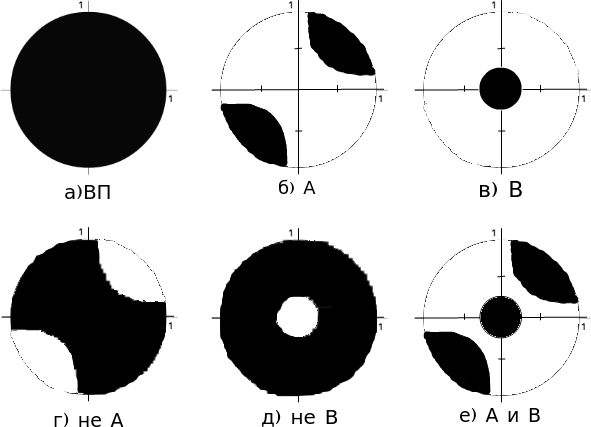
\includegraphics[width=.7\textwidth]{./pictures/2_18.png}
  \caption{Вероятностное пространство и события из задачи 2.18}
  \label{fig:218}
\end{figure}

а) $ A =
\{ (x, y), x^2 + y^2 \leq 1, xy \leq \frac{ 1 }{ 8 } \} $ (\ref{fig:218}, б));

б) $ B =
\{ (x, y), x^2 + y^2 < \frac{ 1 }{ 4 } \} $ (\ref{fig:218}, в));

в) событие $ \overline{ A } $ означает, что событие А не произошло, то есть произведение координат точки превышает 1/8 (\ref{fig:218}, г)):
$$ \overline{ A } =
\{ (x, y), xy > 1/8, x^2 + y^2 \leq 1 \}.$$

Событие $ \overline{ B } $ означает, что точка не оказалась внутри круга радиуса 1/4 (\ref{fig:218}, д)):
$$ \overline{ B } =
\{ (x, y), 1 \geq x^2 + y^2 > \frac{ 1 }{ 4 } \}.$$

Событие $ A \cap B $ означает, что произошло и событие A, и событие B.
Отсюда имеем, что произведение координат точки не должно превышать 1/8, а сумма квадратов координат должна быть меньше 1/4 (\ref{fig:218}, е)), т.е.
$$ A \cap B =
\{ (x, y), x^2 + y^2 < \frac{ 1 }{ 4 }, xy \leq \frac{ 1 }{ 8 } \}.$$

\addcontentsline{toc}{chapter}{Занятие 3. Классическое определение вероятности}
\chapter*{Занятие 3. Классическое определение вероятности}

\addcontentsline{toc}{section}{Контрольные вопросы и задания}
\section*{Контрольные вопросы и задания}

\subsubsection*{Приведите определение вероятностного эксперимента, вероятностного пространства, случайного события.}

Вероятностным экспериментом называется явление, исход которого для нас не определён, и который можно повторить любое число раз независимым образом.

Вероятностное пространство --- совокупность всех исходов вероятностного эксперимента, $\Omega$.

Случайное событие --- подмножество всех исходов вероятностного эксперимента.

\subsubsection*{Как вычислить вероятность события в случае, когда вероятностное пространство состоит из конечного количества равновероятных элементарных событий?}

В этом случае вероятность любого события A вычисляется по формуле
$$ P(A) =
\frac{ |A| }{ |\Omega| },$$
называемой классическим определением вероятности.

\subsubsection*{Запишите формулу включений и исключений.}

Если
$ B_1, B_2,  \dotsc , B_m $ --- некоторые события, то имеет место равенство
$ P\{ \bigcup \limits_{i=1}^m B_i \} =
\sum \limits_{i=1}^m P \{ B_i \} -
\sum \limits_{ 1 \leq i_1 < i_2 \leq m } \{ B_{ i_1 } \cap B_{ i_2 } \} + \dotsc + \\
+ (-1)^{k-1} \sum \limits_{ 1 \leq i_1 < i_2 < \dotsc < i_k \leq m } P \{ B_{ i_1 } \cap B_{ i_2 } \cap \dotsc \cap B_{ i_k } \} + \dotsc + \\
+ (-1)^{m-1} P \{ B_1 \cap B_2 \cap \dotsc \cap B_m \}.$

\addcontentsline{toc}{section}{Аудиторные задачи}
\section*{Аудиторные задачи}

\subsubsection*{3.3}

\textit{Задание.} Пусть A и B такие события, что
$$P \left( A \cap B \right) = \frac{1}{4},
P \left( \overline{A} \right) = \frac{1}{3},
P \left( B \right) = \frac{1}{2}. $$
Вычислите $P \left( A \cup B \right)$.

\textit{Решение.} Вычислим вероятность события A:
$$P \left( A \right) =
1 - P \left( \overline{A} \right) =
1 - \frac{1}{3} =
\frac{2}{3}.$$

Так как события независимы, то вероятность пересечения событий равна произведению пересечений, т.е
$P \left( A \cap B \right) = P \left( A \right) P \left( B \right) $.

Вычислим вероятность объединения:
$$P \left( A \cup B \right) =
P \left( A \right) + P \left( B \right) - P \left( A \cap B \right) =
\frac{2}{3} + \frac{1}{2} - \frac{1}{4} =
\frac{8+6-3}{12} =
\frac{11}{12}.$$

\subsubsection*{3.4}

\textit{Задание.} Было подброшено три монеты.
Найдите вероятности событий:

а) A = {хотя бы одна из монет выпала гербом};

б) B = {выпало ровно два герба};

в) C = {выпало не меньше двух гербов}.

\textit{Решение.} На первой монете может появиться или герб, или цифра.
Аналогичные два элементарных исхода возможны при подбрасывании остальных монет.
Таким образом, общее число возможных элементарных исходов испытания равно $2 \cdot 2 \cdot 2 = 8$.
Эти исходы равновероятны.

а) Благоприятствующие интересующему нас событию
(хотя бы одна из монет выпала гербом)
являются следующие три исхода (<<Г>> означает герб, <<Ц>> --- цифра): 1) ГЦЦ, 2) ГГЦ, 3) ГГГ.

Искомая вероятность равна отношению числа исходов, благоприятствующих событию, к числу всех возможных элементарных исходов:
$$P \left( A \right) =
\frac{3}{8}.$$

б) Благоприятствующим интересующему нас событию (выпало ровно два герба) является следующий исход: ГГЦ.

Искомая вероятность равна
$$P \left( B \right) =
\frac{1}{8}.$$

в) Благоприятствующие интересующему нас событию (выпало не меньше двух гербов) являются следующие два исхода: 1) ГГЦ, 2) ГГГ.

Искомая вероятность равна
$$P \left( C \right) =
\frac{2}{8} =
\frac{1}{4}.$$

\subsubsection*{3.5}

\textit{Задание.} Подброшено 12 игральных кубиков.
Найдите вероятность того, что каждое из очков $1, 2, \dotsc, 6$ выпало дважды.

\textit{Решение.}
На выпавшей грани <<первого>> игрального кубика может появиться одно очко, два очка, $ \dotsc $, шесть очков.
Аналогичные шесть элементарных исходов возможны при бросании остальных кубиков.
Таким образом, общее число возможных элементарных исходов испытания равно $6 \cdot 6 \cdot \dotsc \cdot 6 = 6^{12}$.
Эти исходы в силу симметрии кубиков равновероятны.

Благоприятствующим интересующему нас событию
(каждое из очков выпадет дважды)
является $C_{12}^2 \cdot C_{10}^2 \cdot C_8^2 \cdot C_6^2 \cdot C_4^2 \cdot C_2^2$ исходов.

Искомая вероятность равна отношению числа исходов, благоприятствующих событию,
к числу всех возможных элементарных исходов:
$$P =
\frac{C_{12}^2 \cdot C_{10}^2 \cdot C_8^2 \cdot C_6^2 \cdot C_4^2 \cdot C_2^2}{6^{12}}.$$

\subsubsection*{3.6}

\textit{Задание.}
Игральный кубик изготовлено так,
что вероятность выпадения каждой грани пропорциональна количеству очков, изображённой на этой грани.
Вычислите вероятность того, что при подбрасывании такого игрального кубика выпадет чётное количество очков.

\textit{Решение.} Вероятность выпадения единицы пропорциональна единице, т.е. равна n, где n --- любое натуральное число.
Вероятность выпадения двойки равна $2 n$, тройки --- $3 n$, четвёрки --- $4 n$, пятёрки --- $5 n$ и шестёрки --- $6 n$.
Вероятность выпадения хоть какого-то числа равна единице, т.е. сумма вероятностей выпадения всех граней равна единице: $n + 2 n + 3 n + 4 n + 5 n + \\ + 6 n = 21 n = 1$.
Отсюда
$$n =
\frac{1}{21}.$$

Интересующие нас события: выпадет 2 очка, 4 очка или 6 очков.
2 очка может выпасть с вероятностью
$$ P \left( 2 \right) =
2 \cdot \frac{1}{21} =
\frac{2}{21}.$$
4 очка может выпасть с вероятностью
$$ P \left( 4 \right) =
4 \cdot \frac{1}{21} =
\frac{4}{21}.$$
6 очков может выпасть с вероятностью
$$ P \left( 6 \right) =
6 \cdot \frac{1}{21} =
\frac{6}{21}.$$

Вероятность выпадения чётного числа равна сумме вероятностей их выпадения:
$$P \left( 2, 4, 6 \right) =
\frac{2}{21} + \frac{4}{21} + \frac{6}{21} =
\frac{12}{21}.$$

\subsubsection*{3.7}

\textit{Задание.} Найдите вероятность того, что наугад выбранное число из множества $\{ 1, 2, \dotsc, 100!\}$ делится:

а) на 2;

б) на 2 и на 3;

в) хотя бы на одно из чисел 2, 3, или 5.

\textit{Решение.} Всего чисел $100!$.

а) На 2 делится каждое второе число, т.е. количество чисел, которые делятся на 2, равно
$$\frac{100!}{2}.$$
Вероятность выбора чётного числа равна
$$P =
\frac{ \frac{100!}{2} }{100!} =
\frac{1}{2}.$$

б) На 2 и на 3 делится каждое шестое число, т.е. их всего
$$ \frac{100!}{6}.$$
Тогда вероятность выбора числа, которое делится и на 2, и на 3, равна
$$P =
\frac{ \frac{100!}{6} }{100!} =
\frac{1}{6}.$$

в) На 2 делится каждое второе число, на 3 --- каждое третье, на 5 --- каждое пятое.
Используем формулу включений-исключений:
$$P =
\frac{1}{2} + \frac{1}{3} + \frac{1}{5} - \frac{1}{6} - \frac{1}{10} - \frac{1}{15} + \frac{1}{30} =
\frac{15+10+6-5-3-2+1}{30} =
\frac{22}{30} =
\frac{11}{15}.$$

\subsubsection*{3.8}

\textit{Задание.} В лифт девятиэтажного дома зашло пятеро человек.
Известно, что каждый из них с одинаковой вероятностью может выйти на любом этаже, начиная со второго.
Найдите вероятность того, что:

а) все пятеро выйдут на 5-м этаже;

б) все пятеро выйдут на одном и том же этаже;

в) все пятеро выйдут на разных этажах;

г) двое людей выйдут на 4-м этаже, двое --- на 7-м и один человек выйдет на 9-м этаже.

\textit{Решение.} Каждый из пяти человек может выйти на любом из восьми этажей.
Тогда всего есть $8 \cdot 8 \cdot 8 \cdot 8 \cdot 8 = 8^5$ вариантов.

а) Все пять человек могут выйти на пятом этаже одним способов.
Тогда вероятность этого события равна
$$P =
\frac{1}{8^5}.$$

б) Все пять человек могут выйти на одном и том же этаже восемью способами.
Тогда вероятность этого события равна
$$P =
\frac{8}{8^5} =
\frac{1}{8^4}.$$

в) Первый человек может выйти на любом из восьми этажей, второй --- на любом из оставшихся семи,
третий --- на любом из оставшихся шести, четвёртый --- пяти, и наконец пятый --- на оставшихся четырёх этажах.
Тогда вероятность равна
$$P =
\frac{8 \cdot 7 \cdot 6 \cdot 5 \cdot 4}{8^5} =
\frac{7 \cdot 6 \cdot 5 \cdot 4}{8^4}.$$

г) На четвёртом этаже могут выйти 2 человека из пяти $ \left( C_5^2 \right) $.
На седьмом этаже --- двое из оставшихся трёх человек.
Это $C_3^2$.
На девятом --- один человек из одного.
Это один способ.
Тогда вероятность равна
$$P =
\frac{C_5^2 \cdot C_3^2}{8^5}.$$

\subsubsection*{3.9}

\textit{Задание.} Из колоды карт наугад выбирают 3 карты (без возвращения).
Найдите вероятность того, что среди этих карт:

а) окажется ровно одни туз;

б) окажется хотя бы один туз;

в) окажется тройка, семёрка, туз.

\textit{Решение.} Всего в колоде 52 карты.
Тогда есть 4 масти по 13 карт в каждой.
3 карты из 36 можно выбрать $C_{52}^3$ способами.

а) В колоде есть 4 туза.
Один из них можно выбрать $C_4^1$ способами.
Остаётся выбрать две карты из $52-4=48$.
Это можно сделать $C_{48}^2$ способами.
Тогда вероятность выбрать 3 карты так, что среди них окажется ровно 1 туз, равна
$$P =
\frac{C_4^1 \cdot C_{48}^2}{C_{52}^3}.$$

б) Одной из трёх вытянутых карт должен быть туз.
Выбрать его можно $C_4^1$ способом.
Остальные две карты могут быть любыми.
Их можно выбрать $C_{51}^2$ способами.
Тогда вероятность равна
$$P =
\frac{C_4^1 \cdot C_{51}^2}{C_{52}^3}.$$

в) Есть 4 варианта выбрать тройку, 4 выбрать семёрку и 4 --- туз.
Первой картой может быть тройка, семёрка или туз ($4 \cdot 3 = 12$ карт из 52).
Далее должна быть одна из восьми карт (т.е. 8 вариантов из оставшихся 51 карты).
Последней картой может быть любая из четырёх (из 50 карт).
По правилу произведения имеем
$$P =
\frac{12}{52} \cdot \frac{8}{51} \cdot \frac{4}{50}.$$

\subsubsection*{3.10}

\textit{Задание.} В партии, что состоит из $N$ деталей, есть $M$ бракованных.
Найдите вероятность того, что среди $n \, \left( n < N \right)$ наугад выбранных деталей окажется:

а) $m \, \left( m < M \right) $ бракованных;

б) не больше $m$ бракованных.

\textit{Решение.} Пространство элементарных событий $ \Omega $ является множеством n-элементных подмножеств множества из $N$ элементов.
Значит, $| \Omega | = C_N^n$.

а) Посчитаем число исходов,
благоприятствующих интересующему нас событию
(среди $n$ деталей ровно $m$ бракованных):
$m$ бракованных деталей можно взять из $M$ бракованных деталей $C_M^m$ способами;
при этом остальные $n - m$ деталей не должны быть бракованными;
взять же $n - m$ не бракованных деталей из $N - M$ не бракованных деталей можно $C_{N-M}^{n-m}$ способами.
Следовательно, число благоприятствующих исходов равно $C_M^m C_{N-M}^{n-m}$.

Искомая вероятность равна отношению числа исходов, благоприятствующих событию, к числу всех элементарных исходов:
$$P =
\frac{C_M^m C_{N-M}^{n-m}}{C_N^n}.$$

б) Посчитаем число исходов,
благоприятствующих интересующему нас событию
(среди $n$ деталей от нуля до $m$ бракованных):
от нуля до $m$ бракованных деталей можно взять из $M$ бракованных деталей $ \sum \limits_{i=0}^m C_M^i$ способами;
при этом остальные от $n - m$ до $n$ деталей не должны быть бракованными;
взять же от $n - m$ до $n$ не бракованных деталей из $N - M$ не бракованных деталей можно $ \sum \limits_{i=0}^m C_{N-M}^{n-i}$ способами.
Следовательно, число благоприятствующих исходов равно $ \sum \limits_{i=0}^m C_M^i C_{N-M}^{n-i}$.

Искомая вероятность равна отношению числа исходов, благоприятствующих событию, к числу всех элементарных исходов:
$$P =
\frac{ \sum \limits_{i=0}^m C_M^i C_{N-M}^{n-i}}{C_N^n}.$$

\subsubsection*{3.11}

\textit{Задание.} В купейный вагон (9 купе по 4 места в каждом) семи пассажирам продано семь билетов.
Найдите вероятность того, что занятыми окажутся:

а) ровно два купе;

б) ровно три купе.

\textit{Решение.}
Любой из семи пассажиров может занять любое из четырёх мест в любом из девяти купе (всего мест $4 \cdot 9 = 36$).
Тогда общее число элементарных исходов --- $C_{36}^7$.

а) Для начала необходимо выбрать 2 вагона из девяти.
Это $C_9^2$ способа.
Далее нужно разместить 7 пассажиров среди восьми мест в этих двух вагонах ($C_{8}^7$ способов).
Тогда число благоприятствующих исходов равно $С_9^2 C_8^7$.

Вероятность указанного события равна
$$P =
\frac{С_9^2 C_8^7}{C_{36}^7}.$$

б) Для начала нужно выбрать 3 вагона из девяти.
Это $C_9^3$ способа.
Далее нужно разместить 7 пассажиров среди двенадцати мест в этих трёх вагонах ($C_{12}^7$ способов).
Тогда число благоприятствующих исходов равно $C_9^3 C_{12}^7$.

Вероятность указанного события равна
$$P =
\frac{C_9^3 C_{12}^7}{C_{36}^7}.$$

\subsubsection*{3.12}

\textit{Задание.} Шутник Петя написал письма $n$ адресатам, в каждый конверт вложил по одному письму, а потом наугад написал на каждом из конвертов один из $n$ адресов.
Найдите вероятность того, что:

а) хотя бы одно письмо придёт по назначению;

б) ровно $m$ писем придут по назначению. 

\textit{Решение.} Разложить $n$ писем в $n$ конвертов можно $n!$ способами.

а) Найдём вероятность того, что ни одно письмо не попадёт в конверт с правильным адресом, а затем вычтем её из $1$.

Из общего числа способов необходимо вычесть число тех вариантов, при которых первое письмо попадает в 1-й конверт,
все способы, при которых второе письмо попадает во 2-й конверт и т.д.

Письмо, которое будет вложено в конверт с правильным адресом, можно выбрать $n$ способами;
остальные $n - 1$ письмо можно вложить в $n - 1$ конверт $ \left( n - 1 \right)!$ способами,
поэтому общее число вариантов размещения писем по конвертам равно $n \cdot \left( n - 1 \right)! = n!$.
Вычитая это число из общего числа возможных вариантов размещения писем по конвертам, равного $n!$,
мы не оставляем ни одного варианта.
Вариант, в котором, например, первое письмо попадает в 1-й конверт, а второе письмо --- во 2-й, мы вычитаем дважды.

Чтобы найти, сколько вариантов мы вычли слишком большое число раз, заметим, что существует 
$$C_n^2 =
\frac{n!}{2! \left( n-2 \right)!} =
\frac{n \left( n-1 \right) }{2!}$$
пар писем, и если письма, образующие пару, вложены в конверты с правильными адресами, то остальные $n - 2$ письма можно распределить по конвертам
$$\frac{n \left( n-1 \right)}{2!} \cdot \left( n-2 \right)! =
\frac{n!}{2!}$$
способами.

Прибавив число способов распределения писем в конверты, при которых два письма вложены в свои конверты, мы получим всего
$$n! - n! + \frac{n!}{2!}$$
вариантов размещения писем по конвертам.

Но теперь это слишком много,
так как все варианты, при которых в свои конверты вложены три письма, не были учтены
(мы вычли число таких вариантов трижды, а затем прибавили его столько раз,
сколько пар писем можно образовать из трёх писем, т.е. три раза).
Следовательно, мы должны вычесть число способов, которыми можно вложить в конверты с правильными адресами три письма, т.е.
$$C_n^3 \cdot \left( n-3 \right)! =
\frac{n!}{\left( n-3 \right)! 3!}\cdot \left( n-3 \right)! =
\frac{n!}{3!}$$
способов.

Теперь мы вычли слишком много раз число способов,
которыми можно вложить в конверты с правильными адресами четыре письма и т.д.
Таким образом, число способов, которыми письма можно разложить по конвертам так, что ни одно письмо не окажется в конверте с правильным адресом, равно
$$n! - n! + \frac{n!}{2!} - \frac{n!}{3!} + \dotsc + \left( -1 \right)^{n+1} \left( \frac{1}{n!} \right),$$
а вероятность этого события равна этому числу, делённому на $n!$, т.е. равна числу
$$1 - 1 + \frac{1}{2!} + \dotsc + \left( -1 \right)^{n+1} \frac{1}{n!}.$$
Следовательно, вероятность того, что по крайней мере одно письмо окажется в конверте с правильным адресом, равна
$$P =
1 - \frac{1}{2!} + \frac{1}{3!} - \dotsc + \left( -1 \right)^{n+1} \frac{1}{n!}.$$

б) Найдём вероятность того, что $n - m$ писем не попадут в конверты с правильными адресами, а затем вычтем её из 1.

Письма, которые будут вложены в конверты с правильными адресами,
можно выбрать $C_n^m$ способами;
остальные $n - m$ писем можно вложить в $n - m$ конвертов $ \left( n-m \right)!$ способами,
поэтому общее число вариантов размещения писем по конвертам равно $$C_n^m \cdot \left( n-m \right)!.$$

Аналогично пункту а) получаем, что число способов, которыми письма можно разложить по конвертам так, что ровно $m$ писем окажется в конверте с правильным адресом, равно
$$C_n^m
\left( \left( n-m \right)! - \left( n-m \right)! + \frac{ \left(n-m \right)!}{2!} - \frac{ \left( n-m\right)!}{3!} + \dotsc \right),$$
а вероятность этого события равна этому числу, делённому на $n!$, т.е. равна числу
\begin{equation*}
\begin{split}
C_n^m \cdot \frac{1}{n!}
\left( \left( n-m \right)! - \left( n-m \right)! + \frac{ \left(n-m \right)!}{2!} - \frac{ \left( n-m\right)!}{3!} + \dotsc \right) = \\
= \frac{1}{m! \left( n-m \right)!}
\left( \left( n-m \right)! - \left( n-m \right)! + \frac{ \left(n-m \right)!}{2!} - \frac{ \left( n-m\right)!}{3!} + \dotsc \right) = \\
= \frac{1}{m!} \left( \frac{1}{2!} - \frac{1}{3!} + \dotsc \right).
\end{split}
\end{equation*}

Следовательно, вероятность того, что ровно $m$ писем окажется в конвертах с правильными адресами, равна
$$P =
1 - \frac{1}{m!} \left( \frac{1}{2!} - \frac{1}{3!} + \dotsc \right).$$

\paragraph*{Число встреч}

В задаче используется понятие <<число встреч>>.
Под ним понимается число перестановок множества $\{ 1, \dotsc, n \}$ с заданным числом неподвижных элементов.
Для $n \geq 0$ и $0 \leq k \leq n$ число встреч $D_{n, k}$ --- это число перестановок $\{ 1, \dotsc, n \}$,
содержащих ровно $k$ элементов, не изменивших положение в перестановке.

\begin{figure}[h!]
  \centering
  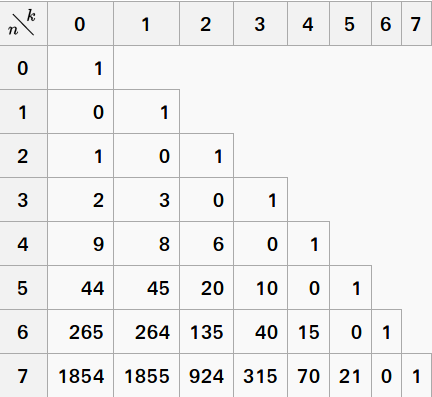
\includegraphics[width=.7\textwidth]{./pictures/3_12.png}
  \caption{Фрагмент таблицы числа встреч}
  \label{fig:312}
\end{figure}

Числа в первом столбце $ \left( k=0 \right) $ показывают число беспорядков (рис. \ref{fig:312}).
Так,
$D_{0, 0} = 1, D_{1, 0} = 0, D_{n+2, 0} = \left( n+1 \right) \left( D_{n+1, 0} + D_{n, 0} \right)$ для неотрицательного $n$.

Выберем $m$ фиксированных элементов из $n$, затем посчитаем число беспорядков оставшихся $n - m$ элементов.
Это будет
$$ \left( n-m \right)! \sum \limits_{k=0}^{n-m} \frac{ \left( -1 \right)^k}{k!}.$$

$$D_{n ,m} =
C_n^m D_{n-m, 0} =
\frac{n!}{m!} \sum \limits_{k=0}^{n-m} \frac{ \left( -1 \right)^k}{k!}.$$

\subsubsection*{3.13}

\textit{Задание.} (Статистика Максвелла-Больцмана). Каждая из $n$ разных частиц наугад попадает в одну из $N$ ячеек.

а) Найдите вероятность того, что в первой, второй и т.д., N-ой ячейке будет соответственно $n_1, n_2, \dotsc, n_N$ частиц.

б) Найдите вероятность $p_k$ того, что данная ячейка содержит $k$ частиц.

в*) Докажите, что если $n$ и $N$ стремятся к бесконечности так, что
$$ \frac{n}{N} \rightarrow \lambda,$$
то
$$p_k \rightarrow \frac{ \lambda^k}{k!}e^{- \lambda}.$$

г) Найдите вероятность того, что в каждой ячейке есть хотя бы одна частица.

д) Найдите вероятность того, что занято ровно $r$ ячеек.

\textit{Решение.} В случаях а), б) и д) вероятность желаемого события оценивается по формуле
$$p =
\frac{r}{m}.$$
Для каждой из $n$ разных частиц есть $N$ вариантов попасть в одну из ячеек.
Поэтому по правилу умножения имеем общее количество вариантов $m = N^n$.
Вычислим количество $r$ вариантов, что отвечают каждому из событий, указанных в условии задачи.

а) Существует $C_n^{n_1}$ способов, которыми можно отобрать $n_1$ частицу в первую ячейку.
Аналогично, количество способов отобрать $n_2$ частицы во вторую ячейку среди $n - n_1$ частицы, которые остались, равно $C_{n-n_1}^{n_2}$.
Подобным же образом отбираются частицы и для других ячеек.
Поэтому событию способствуют
\begin{equation*}
\begin{split}
r =
C_n^{n_1} \cdot C_{n-n_1}^{n_2} \cdot C_{n - n_1 - n_2}^{n_3} \cdot \dotsc = \\
= \frac{n!}{n_1! \left( n-n_1 \right)!}
\cdot \frac{ \left( n-n_1 \right)!}{n_2! \left( n - n_1 - n_2 \right)!}
\cdot \frac{ \left( n - n_1 - n_2 \right)!}{n_3! \left( n - n_1 - n_2 - n_3 \right)!} \cdot \dotsc = \\
= \frac{n!}{n_1! n_2! n_3! \dotsc n_N!}
\end{split}
\end{equation*}
способов.

Тогда вероятность равна
$$p =
\frac{\frac{n!}{n_1! n_2! n_3! \dotsc n_N!}}{N^n} =
\frac{n!}{N^n \cdot n_1! n_2! n_3! \dotsc n_N!}.$$

б) Сначала нужно отобрать $k$ частиц в фиксированную ячейку
(это можно сделать $C_n^k$ способами),
а потом $n - k$ частиц распределить среди $N - 1$ ячейки
($ \left( N - 1\right)^{n-k}$ способов).
По правилу умножения имеем $r = C_n^k \cdot \left( N-1 \right)^{n-k}$ способов.

Тогда вероятность равна
$$p_k =
\frac{C_n^k \cdot \left( N-1 \right)^{n-k}}{N^n}.$$

в*) Распишем $p_k$:
\begin{equation*}
\begin{split}
p_k =
\frac{C_n^k \left( N-1 \right)^{n-k}}{N^n} =
\frac{n! \left( N-1 \right)^{n-k}}{k! \left( n-k \right)! \cdot N^n} = \\
= \frac{n! \left( N-1 \right)^n}{k! \left( n-k \right)! \cdot N^n \left( N-1 \right)^k} =
\frac{n!}{k! \left( n-k \right)! \left( N-1 \right)^k} \cdot \left( \frac{N-1}{N} \right)^n = \\
= \frac{ \left( n-k \right)! \left( n-k+1 \right) \dotsc n}{k! \left( n-k \right)! \left( N-1 \right)^k} \cdot \left(\frac{N-1}{N} \right)^n =
\frac{ \prod \limits_{i=0}^{k-1} \left( n-i \right) }{k! \left( N-1 \right)^k} \cdot \left( \frac{N-1}{N} \right)^n = \\
= \frac{ \prod \limits_{i=0}^{k-1} \left( \frac{n-i}{N-1} \right)}{k!} \cdot \left( 1 - \frac{1}{N} \right)^n.
\end{split}
\end{equation*}

Умножим и поделим последнюю скобку на $n$.
Получим:
\begin{equation*}
\begin{split}
p_k =
\frac{ \prod \limits_{i=0}^{k-1} \left( \frac{n-i}{N-1} \right)}{k!} \cdot \left( 1 - \frac{ \frac{n}{N} }{n} \right)^n.
\end{split}
\end{equation*}

Возьмём предел полученного выражения при 
$$ \frac{n}{N} \rightarrow \lambda.$$
Получим:
$$ \lim \limits_{ \frac{n}{N} \rightarrow \lambda } p_k =
\lim \limits_{ \frac{n}{N} \rightarrow \lambda }
\left( \frac{ \prod \limits_{i=0}^{k-1} \left( \frac{n-i}{N-1} \right)}{k!} \cdot \left( 1 - \frac{ \frac{n}{N} }{n} \right)^n \right) =
\frac{ \lambda^k}{k!} \exp \left( - \lambda \right).$$

г) Вероятность соответственного события вычисляется с помощью формулы включений и исключений:
$P \left\{ \bigcup \limits_{i=1}^m B_i \right\} =
\sum \limits_{i=1}^m P \left\{ B_i \right\} - \\
- \sum \limits_{1 \leq i_1 < i_2 \leq m} P \left\{ B_{i_1} \cap B_{i_2} \right\} + \dotsc + \\
+ \left( -1 \right)^{k-1} \sum \limits_{1 \leq i_1 < i_2 < \dotsc < i_k \leq m} P \left\{ B_{i_1} \cap B_{i_2} \cap \dotsc \cap B_{i_k} \right\} + \dotsc + \\
+ \left( -1 \right)^{m-1} P \left\{ B_1 \cap B_2 \cap \dotsc \cap B_m \right\}$.
Обозначим через $B_i$ событие <<ячейка $i$ не содержит частиц>>.
Тогда $p = 1 - P \left\{ \bigcup \limits_{i=1}^N B_i \right\}$.
Для любых $i = 1, \dotsc, N, \, 1 \leq \\
\leq i_1 < i_2 < \dotsc i_j \leq N$
$$P \left\{ B_i \right\} =
\frac{ \left( N-1 \right)^m}{N^m}, \,
P \left\{ B_{i_1} \cap B_{i_2} \cap \dotsc \cap B_{i_j} \right\} =
\frac{ \left( N-j \right)^m}{N^m}, \,
j = 2, 3, \dotsc, N-1$$
($j$ ячеек являются пустыми; $m$ разных частиц можно разместить в $N - j$ ячейках $ \left( N-j \right)^m$ способами).
Количество слагаемых в соответствующей сумме равно $C_n^j$.
Согласно с формулой включений и исключений имеем окончательный ответ
$$p =
1 - \frac{1}{N^m} \cdot \left[ C_N^1 \cdot \left( N-1 \right)^m - C_N^2 \cdot \left( N-2 \right)^m + \dotsc + \left( -1 \right)^N \cdot C_N^{N-1} \cdot 1^m \right].$$

д) Решение задачи разбиваем на два шага: сначала выбираем $r$ ячеек из $N$, которые будут занятыми (это можно сделать $C_N^r$ способами),
а потом размещаем $n$ разных частиц в $r$ ячеек таким образом, чтобы ни одна из них не была пустой ( подобная задача решена в пункте г) по формуле включений и исключений).
Поэтому окончательно имеем
$r =
C_N^r \times \\
\times \left[ r^n - C_r^1 \cdot \left( r-1 \right)^n + C_r^2 \cdot \left( r-2 \right)^n - \dotsc + \left( -1 \right)^{r-1} \cdot C_r^{r-1} \cdot 1^n \right]$.

\addcontentsline{toc}{section}{Дополнительные задачи}
\section*{Дополнительные задачи}

\subsubsection*{3.14}

\textit{Задание.} Каждое из двух чисел $a, b$ наугад выбирают из множества $ \left\{ 1, 2, \dotsc, n \right\}$.
Вычислите вероятность того, что одно из них делится на другое.
Найдите предел этой вероятности при $n \rightarrow \infty$.

\textit{Решение.} Вероятность будет равна
$$P =
\frac{k}{m},$$
где $k$ --- сумма количества делителей каждого числа из множества  $ \left\{ 1, 2, \dotsc, n \right\}$, $m$ --- количество разных пар чисел.

Найдём $m$.
Это будет число комбинаций из $n$ по $2$: $C_n^2$.

Найдём количество множителей натурального числа.
Пусть
$n =
p_1^{ \alpha_1} \cdot p_2^{ \alpha_2} \cdot \\
\cdot \dotsc \cdot p_s^{ \alpha_s}$
--- каноническое разложение на простые множители натурального числа $n$.
Тогда число $ \tau \left( n \right) $ натуральных делителей числа $n$ выражается формулой
$ \tau \left( n \right) =
\left( \alpha_1 + 1 \right) \dotsc \left( \alpha_s + 1 \right)$.

Каждый натуральный делитель $d$ числа $n$
может быть записан в виде
$d = p_1^{ \delta_1} p_2^{ \delta_2} \dotsc p_s^{ \delta_s}$, где $ \delta_i$ ---
целые числа, удовлетворяющие условиям
$ \delta_i \in  \\
\in \left\{ 0, 1, \dotsc, \alpha_i \right\}$
для $i = 1, 2, \dotsc, s$.

Докажем это утверждение.
Пусть $d$ есть какой-либо натуральный делитель $n$.
Так как каждый простой делитель числа $d$
является делителем числа $n$, то ввиду
$n =
p_1^{ \alpha_1} \cdot p_2^{ \alpha_2} \cdot \dotsc \cdot p_s^{ \alpha_s}$
в разложении $d$ на простые множители могут встречаться только числа множества $ \left\{ p_1, \dotsc, p_s \right\}$.
Поэтому число $d$ представимо в виде $d = p_1^{ \delta_1} p_2^{ \delta_2} \dotsc p_s^{ \delta_s}$, где $ \delta_i$,
причём показатели $ \delta_i$ должны удовлетворять условиям
$ \delta_i \in \left\{ 0, 1, \dotsc, \alpha_i \right\}$ для $i = 1, 2, \dotsc, s$.

С другой стороны, если $d$ представимо в виде
$d =
p_1^{ \delta_1} p_2^{ \delta_2} \dotsc p_s^{ \delta_s}$
и показатели удовлетворяют условиям
$ \delta_i \in \left\{ 0, 1, \dotsc, \alpha_i \right\}$
для $i = 1, 2, \dotsc, s$, то
$n =
d \left( p_1^{ \alpha_1 - \delta_1} \dotsc p_s^{ \alpha_s - \delta_s} \right) \left( \alpha_i - \delta_i \geq 0 \right)$,
т.е. $d$ является натуральным делителем числа $n$.

Чтобы найти число всех натуральных делителей числа $n$,
достаточно посчитать число всевозможных упорядоченных наборов
$ \delta_1, \dotsc, \delta_s$, удовлетворяющих условиям
$ \delta_i \in \left\{ 0, 1, \dotsc, \alpha_i \right\}$ для $i = 1, 2, \dotsc, s$.
Ввиду условий $ \delta_i$ может принимать $ \alpha_i + 1$ значение,
выборы различных значений $ \delta_1, \dotsc, \delta_s$
не зависят один от другого
и в силу единственности разложения на простые множители разным наборам соответствуют различные делители $n$.
Следовательно, число всех натуральных делителей числа $n$ равно
$ \left( \alpha_1 + 1 \right) \dotsc \left( \alpha_s + 1 \right)$.

Можно оценить количество делителей числа.
В терминах о-малое,
функция делителей удовлетворяет неравенству для всех $ \epsilon > 0, \, d \left( n \right) = o \left( n^{\epsilon} \right)$.

Тогда имеем вероятность
$$P =
\frac{ \sum \limits_{i=1}^n i^{\epsilon}}{C_n^2} \, \forall \epsilon > 0.$$

\addcontentsline{toc}{section}{Домашнее задание}
\section*{Домашнее задание}

\subsubsection*{3.15}

\textit{Задание.} Докажите, что для произвольных событий A и B
$ P( AB ) = \\
= 1 - P\left( \overline{ A } \right) - P \left( \overline{ B } \right) + P \left( \overline{ A } \, \overline{ B } \right) $.

\textit{Решение.}
$ P( AB ) =
P(A) + P(B) - P \left( A \cup B \right) = \\
= 1 - P \left( \overline{ A }\right) + 1 - P \left( \overline{ B } \right) - \left( 1 - P \left( \overline{ A \cup B } \right) \right) =
1 - P \left( \overline{ A } \right) + 1 - P \left( \overline{ B } \right) - 1 + P \left( \overline{ A } \, \overline{ B } \right) = \\
= 1 - P \left( \overline{ A } \right) - P \left( \overline{ B } \right) + P \left( \overline{ A } \, \overline{ B } \right) $.

\subsubsection*{3.16}

\textit{Задание.} Подбрасывают 4 игральных кубика.
Найдите вероятность того, что на них выпадет одинаковое количество очков.

\textit{Решение.} На выпавшей грани <<первого>> игрального кубика может появиться одно очко, два очка,  $ \dotsc $ , шесть очков.
Аналогичные шесть элементарных исходов возможны при бросании остальных кубиков.
Таким образом, общее число возможных элементарных исходов испытания равно $ 6 \cdot 6 \cdot 6 \cdot 6 = 1296 $.
Эти исходы в силу симметрии кубиков равновероятны.

Благоприятствующие интересующему нас событию
(на всех гранях появится одинаковое количество очков)
являются следующие шесть исходов
(первым записано число очков,
выпавших на <<первом>> кубике,
вторым --- число очков, выпавших на <<втором>> кубике, и т.д.): 1) 1, 1, 1, 1, 2) 2, 2, 2, 2, 3) 3, 3, 3, 3, 4) 4, 4, 4, 4, 5) 5, 5, 5, 5, 6) 6, 6, 6, 6.

Искомая вероятность равна отношению числа исходов, благоприятствующих событию, к числу всех возможных элементарных исходов:
$$ P =
\frac{6}{6^4} = \frac{1}{6^3}.$$

\subsubsection*{3.17}

\textit{Задание.} Группа состоит из r студентов.
Найдите вероятность того, что по крайней мере 2 студента родились в одном и том же месяце (считайте, что все месяцы года являются равновероятными для рождения).

\textit{Решение.} Год имеет 12 месяцев.
День рождения каждого из студентов может приходиться на любой месяц года (12 вариантов).

Если студентов больше чем месяцев ($ r > 12 $), то не существует исходов, при которых в один месяц попадает один человек.
$ P = 0 $.

Рассмотрим случай, когда студентов в группе не больше чем месяцев в году ($ r \leq 12 $).
По правилу умножения существует всего $ n = 12^r $ вариантов размещения дней рождения студентов.
Найдём количество вариантов, когда никакие два студента не имеют день рождения в тот же месяц.
Для этого нужно вычислить количество способов, которыми из 12 месяцев можно выбрать упорядоченное множество из r месяцев.
Используя формулу для размещения из 12 элементов по r, имеем $ A_{12}^r $.
Поэтому
$$ P =
1 - \frac{ A_{ 12 }^r }{ 12^r }.$$

\subsubsection*{3.18}

\textit{Задание.} Сколько людей должно быть в комнате, чтобы вероятность того, что хотя бы двое из присутствовавших родились в один и тот же день года, была большей чем 1/2?

\textit{Решение.} Пусть r --- число людей, и будем считать, что все дни рождения равновероятны.
Вычислим вероятность противоположного события A = {все люди родились в разные дни}.
Число способов, благоприятствующих этому событию --- это число размещений из 365 по r.
Всего же имеется $ n = 365^r $ возможностей распределения дней рождения.
То есть
$$ P(A) =
\frac{A_{365}^r}{365^r}.$$

Вероятность интересующего нас события $ \overline{A} $ тогда равна
$$ P \left( \overline{A} \right) =
1 - P \left( A \right) =
1 - \frac{A_{365}^r}{365^r}.$$

Вычислим вероятность $ P \left( \overline{A} \right) $ для различных значений r.
\begin{equation*}
\begin{split}
r = 5 : P \left( \overline{A} \right) =
1 - \frac{A_{365}^5}{365^5} =
1 - \frac{5! \cdot C_{365}^5}{365^5} = \\
= 1 - \frac{5! \cdot \frac{365!}{5! \cdot 360!} }{365^5} =
1 - \frac{365!}{360! \cdot 365^5} =
1 - \frac{360! \cdot 361 \cdot 362 \cdot 363 \cdot 364 \cdot 365}{360! \cdot 365^5} = \\
= 1 - \frac{361 \cdot 362 \cdot 363 \cdot 364}{365^4} =
1 - \frac{1.72 \cdot 10^10}{1.77 \cdot 10^10} =
1 - 0.97 =
0.03.
\end{split}
\end{equation*}

\begin{equation*}
\begin{split}
r = 10 :
P \left( \overline{A} \right) =
1 - \frac{A_{365}^{10}}{365^{10}} =
1- \frac{10! \cdot C_{365}^{10}}{365^{10}} = \\
= 1 - \frac{10! \cdot \frac{365!}{10! \cdot 355!}}{365^{10}} =
1 - \frac{365!}{355! \cdot 365^{10}} =
0.12.
\end{split}
\end{equation*}

\begin{equation*}
\begin{split}
r = 20 :
P \left( \overline{A} \right) =
1 - \frac{A_{365}^{20}}{365^{20}} =
1 - \frac{20! \cdot C_{365}^{20}}{365^{20}} =
1 - \frac{365!}{345! \cdot 365^{20}} =
0.41.
\end{split}
\end{equation*}

\begin{equation*}
\begin{split}
r = 22 :
P \left( \overline{A} \right) =
1 - \frac{A_{365}^{22}}{365^{22}} =
1 - \frac{365!}{343! \cdot 365^{22}} =
0.48.
\end{split}
\end{equation*}

\begin{equation*}
\begin{split}
r = 23 :
P \left( \overline{A} \right) =
1 - \frac{A_{365}^{23}}{365^{23}} =
1 - \frac{365!}{342! \cdot 365^{23}} =
0.51.
\end{split}
\end{equation*}

При
$ r = 23 $
вероятность по крайней мере одного совпадения равна
$ 0.51 > \\
> 0.5 $,
то есть
$ r = 23 $ ---
наименьшее число, удовлетворяющее условиям задачи.

\subsubsection*{3.19}

\textit{Задание.} Числа $ 1, 2,  \dotsc , n $ размещены в случайном порядке.
Найдите вероятность того, что числа:
а) 1 и 2;
б) 1, 2 и 3 размещены рядом в указанном порядке.

\textit{Решение.} Пространство элементарных событий $  \Omega$ является множеством всех перестановок множества из n элементов.
Значит $ |\Omega| = n! $.

а) Поскольку числа 1 и 2 стоят рядом, то их можно рассматривать как одно число (обозначим его $ n + 1 $).
Количество возможных перестановок чисел $ \{ 3, 4,  \dotsc , n + 1 \} $ равно $ \left( n - 1 \right)! $.
Тогда вероятность данного события равна:
$$ P =
\frac{ \left( n - 1 \right)! }{ n! } =
\frac{1}{n};$$

б) поскольку числа 1, 2 и 3 стоят рядом, то их можно рассматривать как одно число (обозначим его $ n + 1 $).
Количество возможных перестановок чисел $ \{ 4, 5,  \dotsc , n + 1 \} $ равно $ \left( n - 2 \right)! $.
Тогда вероятность данного события равна:
$$ P = \frac{ \left( n - 2 \right)!}{ n! } =
\frac{1}{ n (n - 1 ) }.$$

\subsubsection*{3.20}

\textit{Задание.} Экзамен состоит из 10 вопросов, на каждый из которых нужно дать ответ <<да>> или <<нет>>.
Найдите вероятность того, что студент правильно ответил хотя бы на $ 70 \% $ вопросов, выбирая ответ наугад.
Решите задачу, если тест состоит из 30 и из 50 вопросов.

\textit{Решение.} На каждый вопрос есть возможность ответить двумя способами (<<да>> или <<нет>>).

В случае, когда экзамен состоит из десяти вопросов, пространство элементарных событий содержит $ | \Omega | = 2^{10} $ элементов.
Найдём вероятность события А = {студент правильно ответит хотя бы на 70\% вопросов из десяти}.
Ответить правильно хотя бы на 70\% вопросов означает ответить правильно хотя бы на 7 вопросов из 10, т. е. событие А допускает правильный ответ на 7, 8, 9 или 10 вопросов.
На 7 вопросов правильно можно ответить $ C_{10}^7 $ способами.
На 8 вопросов правильно можно ответить $ C_{10}^8 $ способами.
На 9 --- $ C_{10}^9 $.
Аналогично, на 10 вопросов можно дать правильный ответ $ C_{10}^{10} $ способами.
По правилу суммы имеем $ |A| = C_{10}^7 + C_{10}^8 + C_{10}^9 + C_{10}^{10} = \sum \limits_{i=7}^{10} C_{10}^i $.
Тогда вероятность события A равна
$$ P \left( A \right) =
\frac{|A|}{| \Omega |} =
\frac{ \sum \limits_{i=7}^{10} C_{10}^i}{2^{10}}.$$

Аналогично находим вероятность правильного ответа на хотя бы 70\% вопросов из тридцати и пятидесяти.

Когда всего есть 30 вопросов (событие B), то 70\% от них --- это $ 30 \cdot 0.7 = 21$ вопрос.
Тогда
$$ P \left( B \right) =
\frac{ \sum \limits_{i=21}^{30} C_{30}^i}{2^{30}}.$$

Когда всего есть 50 вопросов (событие C), то 70\% от них --- это $ 50 \cdot 0.7 = 35$ вопрос.
Тогда
$$ P \left( C \right) =
\frac{ \sum \limits_{i=35}^{50} C_{50}^i}{2^{50}}.$$

\subsubsection*{3.21}

\textit{Задание.} Список из 4N участников турнира разбито на четыре равные группы.
Найдите вероятность того, что четыре самых сильных участника турнира окажутся в разных группах. 

\textit{Решение.} Найдём сначала количество вариантов, которыми N участников можно выбрать в первую группу.
Для этого достаточно из 4N участников выбрать N, т.е. $ n = C_{4N}^N $.
Выберем того самого сильного участника, который попадёт в первую группу (это можно сделать четырьмя способами).
В эту же группу нужно дополнительно выбрать $ N - 1 $ участника из $ 4N - 4 $ участников, что остались ($ C_{ 4N - 4 }^{ N - 1 } $ способов).
Отсюда следует, что четыре самых сильных участника попадут в разные группы с вероятностью
\begin{equation*}
\begin{split}
p =
\frac{ 4C_{ 4N - 4 }^{ N - 1 } }{ C_{ 4N }^N } =
\frac{ 4 \cdot \frac{ (4N-4)! }{ ( N - 1 )!( 3 N - 3)! } }{ \frac{ (4N)! }{ N!(3N)! } } =
\frac{ 4(4N-4)!N!(3N)! }{ (N-1)!(3N-3)!(4N)! } = \\
= \frac{ 4(4N-4)!(N-1)!N(3N-3)!(3N-2)(3N-1)3N }{ (N-1)!(3N-3)!(4N-4)!(4N-3)(4N-2)(4N-1)4N } = \\
= \frac{ 3N(3N-2)(3N-1) }{ (4N-3)(4N-2)(4N-1) } =
\frac{ 3N(3N-2)(3N-1) }{ 2(4N-3)(2N-1)(4N-1) }.
\end{split}
\end{equation*}

\subsubsection*{3.22}

\textit{Задание.} При игре в покер игрок имеет на руках пять карт из колоды в 52 карты.
Найдите вероятность следующих комбинаций:

а) <<royal flush>> (десятка, валет, дама, король и туз одной масти);

б) <<straight flush>> (пять карт подряд одной масти, но не <<royal flush>>);

в) <<four of a kind>> (четыре карты одного порядка);

г) <<full house>> (2 карты одинакового порядка и 3 карты одинакового порядка);

д) <<flush>> (пять карт одой масти, но не <<royal flush>> и не <<straight flush>>);

е) <<straight>> (пять карт подряд не все одной масти).

\textit{Решение.} Выбрать 5 карт из 52 можно $ C_{52}^5 $ способами.

а) Так как есть 4 масти, то десятку можно выбрать четырьмя способами.
Поэтому вероятность выпадения комбинации <<royal flush>> равна
$$ p =
\frac{ C_4^1 }{ C_{52}^5 };$$

б) есть 9 комбинаций пяти карт подряд одной масти.
Так как мастей 4, то этих комбинаций $ 9 \cdot 4 = 36 $.
Поэтому вероятность комбинации <<straight flush>> равна
$$ p =
\frac{ C_{36}^1 }{ C_{52}^5 }.$$
После исключения комбинации <<royal flush>>, получим
$$ p =
\frac{ C_{36}^1 - C_4^1 }{ C_{52}^5 };$$

в) есть 4 масти, в каждой из которых $ 52 : 4 = 13 $ карт.
Есть 13 способов выбрать 4 карты одного порядка.
Так же нужно дополнительно выбрать одну любую карту из оставшихся $ 52 - 4 = 48 $ карт (это 48 способов).
Отсюда имеем, что вероятность комбинации <<four of a kind>> равна
$$ p =
\frac{ C_{13}^1 \cdot C_{48}^1 }{ C_{52}^5 };$$

г) есть карты тринадцати порядков четырёх мастей.
Две карты одного порядка могут иметь любой из тринадцати порядков и любые две из четырёх мастей (это $ C_{13}^1 \cdot C_4^2 $).
Осталось выбрать 3 карты одного порядка. Имеем теперь 12 порядков карт.
Поэтому есть $ C_{12}^1 \cdot C_4^3 $ способов их выбрать.
Итого имеем, что вероятность комбинации <<full house>> равна
$$ p =
\frac{ C_{13}^1 \cdot C_4^2 \cdot C_{12}^1 \cdot C_4^3 }{ C_{52}^5 };$$

д) пять карт одной масти можно выбрать $ 4 \cdot C_{13}^5 $ способами.
Отнимем из этих комбинаций <<royal flush>> и <<straight flush>>.
Получим $ 4 \cdot C_{13}^5 - С_4^1 - C_{36}^1 $.
Поэтому вероятность комбинации <<flush>> равна
$$ p =
\frac{ 4 \cdot C_{13}^5 - С_4^1 - C_{36}^1 }{ C_{52}^5 };$$

е) имея только одну масть есть 9 комбинаций пяти карт подряд.
Каждая из этих пяти карт может быть любой масти.
Главное, чтобы хотя бы одна карта имела масть, отличающуюся от остальных четырёх карт.
Имеем $ 9 \cdot 4^5 $ комбинаций.
Теперь отнимем от них комбинации, где все карты имеют одну масть (их 9).
Поэтому вероятность <<straight>> равна
$$ p =
\frac{ C_9^1 \cdot 4^5 }{ C_{52}^5 }.$$

\subsubsection*{3.23}

\textit{Задание.} Компьютерный центр имеет три процессора, на которые поступило n заданий.
Каждое задание выполняется на наугад выбранном процессоре.
Найдите вероятность того, что ровно один процессор останется незадействованным.

\textit{Решение.} Используем классическое определение вероятности:
$$ P = \frac{m}{k},$$
где m --- число исходов, благоприятствующих осуществлению события, а n --- число всех равновероятных элементарных исходов.

Посчитаем k.
Представим, что процессор --- это ящик.
Положим ящики рядом.
Две соседние стенки назовём <<перегородкой>>, а две крайние стенки не будем рассматривать.
Тогда у нас будет $ 3 - 1 = 2 $ перегородки.
Ситуация выглядит так: Ящик 1 | Ящик 2 | Ящик 3

В эти ящики кладутся предметы (задания).
Итого у нас $ \left( n + 3 - 1 \right) $ позиция --- для n предметов и двух перегородок.
Задание распределения предметов по ящикам равносильно заданию положения перегородок.
Пусть заданы какие-то две позиции для перегородок,
тогда им соответствует некоторое распределение предметов по ящикам
(при этом некоторые ящики могут оказаться пустыми ---
если какая-то перегородка будет на первом месте,
или на последнем, или какие-то перегородки окажутся на соседних местах).
Если же задано некоторое распределение предметов по ящикам,
то в первом окажется $ n_1 $  предмет
(первая перегородка стоит на
$ \left( n_1 + 1 \right) $-ом месте),
во втором ящике --- $ n_2 $ предмета
(вторая перегородка стоит на
$ \left( n_1 + 1 + n_2 +1 \right) $-ом месте)
и так далее, в итоге получим искомые две позиции для перегородок.

Значит, расположить n предметов по разным ящикам можно
$ k = C_{n+2}^{2} $ способом ---
число различных способов распределить n заданий по 6 процессорам,
причём каждый процессор может получить любое количество заданий.

Теперь посчитаем m.
Заданы 2 разных ящика и n предметов.
Нужно расположить предметы по ящикам так, что ни один ящик не будет пустым.

Используем метод перегородок.
Выложим предметы в ряд.
Нужно расставить перегородки так,
чтобы этот ряд распался на две группы (<<группа>> --- это хотя бы один предмет), соответствующих нашим ящикам.

Между n предметами есть $n-1$ место, на которые можно поставить перегородки.
При каждом расположении этих перегородок, получим искомое разбиение на группы --- и в каждой будет хотя бы одни предмет.
Пусть каким-то образом распределены предметы по ящикам, тогда можем определить положения перегородок между объектами,
учитывая количество объектов в каждом ящике.
Значит,
расположить n предметов по двум различным ящикам так,
что ни один ящик не будет пустым,
можно $ C_{n-1}^1 $ способом ---
число способов распределить n задач на два процессора,
причём каждый процессора должен получить не менее одной задачи.
При этом нужно полученное число сочетаний умножить на 3,
так как процессор, который останется без заданий, можно выбрать 3 способами: $ m = 3 \cdot C_{n-1}^1 $.

Искомая вероятность
$$ P =
\frac{ 3 \cdot C_{n-1}^1 }{ C_{n+2}^{2} }.$$

\subsubsection*{3.24}

\textit{Задание.} (Статистика Бозе-Эйнштейна).
Каждая из n одинаковых частиц наугад попадает в одну из N ячеек.

а) Найдите вероятность того, что в первой, второй и т.д., N-ой ячейке будет соответственно $ n_1, n_2, \dotsc , n_N $ частиц.

б) Докажите, что вероятность $ q_k $ того, что в данной ячейке будет k частиц, равна
$$ q_k =
\frac{ C_{ N+n-k-2 }^{ n-k } }{ C_{ N+n-1 }^n }.$$

в) Докажите, что при $ N > 2 : q_0 > q_1 > q_2 > \dotsc $

г) Докажите, что если n и N стремятся к бесконечности так, что
$$ \frac{ n }{ N } \rightarrow \lambda,$$
то
$$ q_k \rightarrow \frac{ \lambda^k }{ \left( 1 + \lambda \right)^{ k+1 } }.$$

д) Найдите вероятность того, что ровно r ячеек будут пустыми.

\textit{Решение.}

а) Разместим частицы в ряд.
Поставим между ними $ N - 1 $ перегородку.
Обозначим частицу символом <<0>>, а перегородку символом <<1>>.
Тогда распределение частиц однозначно характеризуется последовательностью из n нулей и $ N - 1 $ единицы.
Например, последовательность
$ 1000101100001 \dotsc $
означает, что в первую ячейку попало 3 частицы, во вторую --- одна, в третью не попало ни одной частицы, в четвёртую попало 4 частицы и т.д.
Количество способов, которыми можно распределить n частиц, совпадает с количеством разных последовательностей указанного вида.
Последовательность определяется однозначно, если выбрать $ N - 1 $ место из $ n + N - 1$, где будут размещены единицы.
Количество таких комбинаций равно $ | \Omega | = C_{n+N-1}^{N-1} $.

Событию A = { в первой, второй и т.д., N-ой ячейке окажется соответственно $ n_1, n_2, \dotsc , n_N $ частиц}
способствует одно элементарное событие, а именно
$ \omega_0 = \left( n_1, n_2, \dotsc , n_N \right) $.

Таким образом
$$ P(A) =
\frac{1}{C_{n+N-1}^{N-1}}. $$

б) Вероятность желаемого события оценивается по формуле
$$ q_k =
\frac{r}{| \Omega |}.$$

Аналогично предыдущему пункту $  | \Omega | = C_{n+N-1}^{N-1}  $.

Сначала надо отобрать k частиц в фиксированную ячейку (это можно сделать одним способом), а потом
$ n - k $
частиц распределить среди
$ N - 1 $ ячейки.

Используем метод перегородок.
Разместим все $ n - k $ частиц в ряд.
Чтобы отделить частицы, которые попадут в разные ячейки, поставим между ними $ N - 2 $ перегородки.
Обозначим частицу символом <<0>>, а перегородку символом <<1>>.
Тогда распределение частиц по ячейкам однозначно характеризуется последовательностью из $ n - k $ нулей и $ N - 2$ единиц.
Количество способов, которыми можно распределить
$ n - k $
частиц, совпадает с количеством разных последовательностей указанного вида.
Последовательность определяется однозначно, если выбрать $ N - 2 $ места из $ n - k + N - 2 $, где будут размещены единицы.
Количество таких комбинаций равно $ r = C_{n-k+N-2}^{N-2} $.

Тогда
$$ q_k =
\frac{C_{n-k+N-2}^{N-2}}{C_{n+N-1}^{N-1}}.$$

в) Найдём вероятность $ q_0 $ того, что в данной ячейке будет 0 частиц.
Вероятность желаемого события оценивается по формуле
$$ q_0 =
\frac{r_0}{| \Omega |}.$$

Аналогично пункту а) $  | \Omega | = C_{n+N-1}^{N-1}  $.

Нужно n одинаковых частиц распределить среди $ N - 1 $ ячейки.

Используем метод перегородок.
Разместим все n частиц в ряд.
Чтобы отделить частицы, которые попадут в разные ячейки, поставим между ними $ N - 2 $ перегородки.
Обозначим частицу символом <<0>>, а перегородку символом <<1>>.
Тогда распределение частиц по ячейкам характеризуется последовательностью из n нулей и $ N - 2 $ единиц.
Количество способов, которыми можно распределить n частиц, совпадает с количеством разных последовательностей указанного вида.
Последовательность определяется однозначно, если выбрать $ N - 2 $ места из $ n + N - 2 $, где будут размещены единицы.
Количество таких комбинаций равно $ C_{n+N-2}^{N-2} $.

Тогда
$$ q_0 =
\frac{C_{n+N-2}^{N-2}}{C_{n+N-1}^{N-1}}.$$

Проверим формулу из пункта б).
Подставим $ k = 0 $.
Получим:
$$ q_0 =
\frac{C_{n+N-2}^{N-2}}{C_{n+N-1}^{N-1}}.$$
Видим, что получили такую же формулу, значит для дальнейшего решения можно использовать её, подставляя вместо k нужное значение.

Упростим:
\begin{equation*}
\begin{split}
q_0 =
\frac{ \frac{ \left( n+N-2 \right)! }{ \left( N-2 \right)! \left( n+N-2-N+2 \right)!  } }{ \frac{ \left( n+N-1\right)! }{\left( N-1 \right)! \left( n+N-1-N+1 \right)!  } } =
\frac{ \left( n+N-2\right)! \left( N-1 \right)!n!}{ \left( N-2 \right)!n! \left( n+N-1 \right)! } = \\
= \frac{ \left( n+N-2 \right)! \left( N-2 \right)! \left( N-1 \right) }{ \left( N-2 \right)! \left( n+N-2 \right)! \left( n+N-1 \right) } =
\frac{N-1}{n+N-1}.
\end{split}
\end{equation*}

Упростим общую формулу:
\begin{equation*}
\begin{split}
q_k =
\frac{ \frac{ \left( n-k+N-2 \right)! }{ \left( N-2 \right)! \left( n-k+N-2-N+2 \right)! } }{ \frac{ \left( n+N-1 \right)!}{ \left( N-1 \right)! \left(n+N-1-N+1 \right)!} } =
\frac{ \left( n-k+N-2 \right)! \left( N-1 \right)!n!}{ \left( N-2 \right)! \left( n-k \right)! \left( n+N-1 \right)!} = \\
= \frac{ \left( n-k+N-2 \right)! \left( N-1 \right) n!}{ \left( n-k \right)! \left( n+N-1 \right)!}.
\end{split}
\end{equation*}

Найдём вероятность $ q_1 $ того, что в данной ячейке будет одна частица:
\begin{equation*}
\begin{split}
q_1 =
\frac{ \left( n-1+N-2 \right)! \left( N-1 \right) n!}{ \left( n-1 \right)! \left( n+N-1 \right)!} = \\
= \frac{ \left( n+N-3 \right)! \left( N-1 \right)! \left( n-1 \right)!n }{ \left( n-1 \right)! \left( n+N-3 \right)! \left( n+N-2 \right) \left( n+N-1 \right) } =
\frac{ \left( N-1 \right) n}{ \left( n+N-2 \right) \left( n+N-1 \right).}
\end{split}
\end{equation*}

Сравним $ q_0 $ и $ q_1 $.
Приведём к общему знаменателю.
Для этого $ q_0 $ умножим на $ \left( n+N-2 \right) $.
Получим:
$$ q_0 =
\frac{ \left( N-1 \right) \left( n+N-2 \right) }{ \left( n+N-1 \right) \left( n+N-2 \right) }.$$

Видим, что $ q_0 $ и $ q_1 $ отличаются только выражением в числителе.
Теперь сравним n и $ \left( n+N-2 \right)$.
По условию задачи $ N > 2 $, поэтому $ N - 2 > 0 $.
Это значит, что $ n + N - 2  > n $, т.е. $ q_0 > q_1 $.

Докажем, что условие выполняется для k-го члена.
Найдём вероятность $ q_{k+1} $ того, что в данной ячейке будет $ k + 1 $ частица:
$$ q_{k+1} =
\frac{ \left( n-k-1+N-2 \right)! \left( N-1 \right) n!}{ \left( n-k-1 \right)! \left( n+N-1 \right)!} =
\frac{ \left( n-k+N-3 \right)! \left( N-1 \right) n!}{ \left( n-k-1 \right)! \left( n+N-1 \right)!}.$$

Сравним полученное выражение с $ q_k $.
В выражении для $ q_{k+1} $ и числитель, и знаменатель меньше: $ n - k + N -3 < n - k + N - 2 $, а также $ n - k - 1 < n - k $.
Отсюда следует, что $ q_k > q_{k+1}$.

Итого, доказали, что условие верно для первого члена $ \left( q_0 > q_1 \right) $.
Также из верности условия для k-го члена вытекает его верность для $ k + 1 $-го.
Отсюда по индукции Пеано следует, что условие верно для любого натурального числа.

г) Распишем $ p_k $ (вероятность того, что в данную ячейку попадут k частиц):

\begin{equation*}
\begin{split}
p_k =
\frac{C_{N+n-k-2}^{n-k}}{C_{N+n-1}^n} =
\frac{ \left( N+n-k-2 \right)!n! \left( N-1 \right)!}{ \left( n-k \right)! \left( N-2 \right)! \left( N+n-1 \right)!} = \\
= \frac{ \left( N+n-k-2 \right)! \left( n-k \right)! \left( N-2 \right)! \left( N-1 \right) \prod \limits_{i=0}^{k-1} \left( n-i \right) }{ \left( n-k \right)! \left( N-2 \right)! \left( N+n-k-2 \right)! \prod \limits_{j=1}^{k+1} \left( N+n-j \right) } =
\frac{ \left( N-1 \right) \prod \limits_{i=0}^{k-1} \left( n-i \right) }{ \prod \limits_{j=1}^{k+1} \left( N+n-j \right) }.
\end{split}
\end{equation*}

Поделим числитель и знаменатель на N:
\begin{equation*}
\begin{split}
p_k =
\frac{ \left( 1- \frac{1}{N} \right) \prod \limits_{i=0}^{k-1} \left( \frac{n}{N} - \frac{i}{N} \right) }{ \prod \limits_{j=1}^{k+1} \left( 1+ \frac{n}{N} - \frac{j}{N} \right) } = \\
= \frac{ \frac{n}{N} \left( \frac{n}{N} - \frac{1}{N} \right) \dotsc \left( \frac{n}{N} - \frac{k-1}{N} \right) }{ \left( 1+ \frac{n}{N} - \frac{1}{N} \right) \left( 1+ \frac{n}{N} - \frac{2}{N} \right) \dotsc \left( 1+ \frac{n}{N} - \frac{k+1}{N} \right) } =
\frac{ \lambda^k}{ \left( 1+ \lambda \right)^{k+1}}.
\end{split}
\end{equation*}

д) Вероятность желаемого события оценивается по формуле
$$ p =
\frac{r}{| \Omega |}.$$

Как и в пункте а) имеем общее количество вариантов $ | \Omega | = C_{n+N-1}^{N-1} $.
Вычислим количество вариантов r, которые отвечают событию, указанному в условии задачи.

Решение задачи разбиваем на два шага:
сначала выбираем $ N - r $ ячеек из N, которые будут занятыми (это можно сделать $ C_{N}^{N-r} $ способами),
а затем размещаем n одинаковых частиц в $ N - r $ ячеек таким образом, чтобы ни одна их них не была пустой.
Поскольку все частицы одинаковы, то в каждую ячейку можно заранее поместить по одной частице.
В этом случае задача сводится к распределению $ m - \left( N - r \right) = m - N + r $ частиц на $ N - r $ ячеек.

Используем метод перегородок.
Разместим все частицы в ряд.
Чтобы отделить частицы, которые будут находиться в разных ячейках, поставим между ними $ N - r - 1 $ перегородку.
Обозначим частицу символом <<1>>, а перегородку символом <<0>>.

Тогда распределение частиц по ячейкам характеризуется последовательностью из $ m - N + r $ нулей и $ N - r - 1 $ единицы.
Количество способов, которыми можно распределить $ m - N + r $ частиц, совпадает с количеством разных комбинаций указанного вида.
Последовательность определяется однозначно, если выбрать $ N - r - 1 $ мест из
$ \left( m - N + r \right) + \left( N - r - 1 \right) = \\
= m - N + r + N - r - 1 = m - 1 $,
где будут стоять единицы.
Количество таких комбинаций равно $ C_{m-1}^{N - r - 1} $.

Поэтому окончательно имеем $ r = C_{N}^{N-r} \cdot C_{m-1}^{N - r - 1} $.

Тогда вероятность указанного события равна
$$ p =
\frac{C_{N}^{N-r} \cdot C_{m-1}^{N - r - 1}}{C_{n+N-1}^{N-1}}.$$

\end{document}
